% !TEX TS-program = pdflatex
\documentclass[sigconf]{acmart}

\def\BibTeX{{\rm B\kern-.05em{\sc i\kern-.025em b}\kern-.08emT\kern-.1667em\lower.7ex\hbox{E}\kern-.125emX}}
\usepackage{subfigure}
\usepackage{algorithm}
%\usepackage{algorithmic}
\usepackage{algpseudocode}
\usepackage{amsmath}
\usepackage{graphics}
\usepackage{epsfig}
\usepackage{multirow}
\usepackage{graphicx}
\usepackage{subfigure}


\renewcommand{\algorithmicrequire}{\textbf{Input:}} % Use Input in the format of Algorithm
\renewcommand{\algorithmicensure}{\textbf{Output:}} % Use Output in the format of Algorithm

\begin{document}

\title{Approximate Code: A Cost-Effective Erasure Coding Framework for Tiered Video Storage in Cloud Systems}

\author{Huayi Jin}


%-------------------------ATTANTION-------------------------%
%                                                           %
% orange words show the content that requires to be add     %
% blue words need to be perfected or changed                %
% gray words are the placeholder which is easy to fill      %
%                                                           %
%-----------------------------------------------------------%

\begin{abstract}
Nowadays massive video data are stored in cloud storage systems, which are generated by various applications such as autonomous driving, news media, security monitoring, etc. Meanwhile, erasure coding is a popular technique in cloud storage to provide both high reliability with low monetary cost, where triple disk failure tolerant arrays (3DFTs) is a typical choice. Therefore, how to minimize the storage cost of video data in 3DFTs is challenge for cloud storage systems. Although there are several solutions like approximate storage technique for storage devices, it cannot guarantee low storage cost and high data reliability in storage systems concurrently.

To address this problem, in this paper, we propose Approximate Code, which is an erasure coding framework for video applications in cloud storage systems. The key idea of Approximate Code is distinguishing the important data and unimportant data in videos with different capabilities of fault tolerance. On one hand, for important data, Approximate Code provides triple parities to provide high reliability. On the other hand, single/double parities are applied for unimportant data, which can save the storage cost and accelerate the recovery process. To demonstrate the effectiveness of Approximate Code, we conduct several experiments in Hadoop systems. The results show that, compared to traditional 3DFTs using various erasure codes such as RS, STAR and TIP-Code, Approximate Code reduces the number of parities by up to 60\%, saves the storage cost by up to 10\%, increase the recovery speed by up to 1.5X when single disk fails, and can reconstruct the whole video data via fuzzification when triple disks fail.
                                                                    q
\end{abstract}

%
% The code below is generated by the tool at http://dl.acm.org/ccs.cfm.
% Please copy and paste the code instead of the example below.
%
\keywords{Erasure Codes, Approximate Storage, Multimedia, Cloud Storage}

\maketitle

\section{Introduction}
For typical cloud storage systems such as Windows Azure [CITE] and Amazon AWS [CITE], erasure coding is a popular technique to provide both high reliability and low monetary cost [CITE EC], where triple disk failure fault tolerant arrays (3DFTs) are widely used. Typical erasure codes can be divided into two categories, RS-based Codes [CITE] and XOR-based codes [CITE]. RS-based codes [CITE] are encoded according the Galois Field Computation in Reed Solomon Code [CITE], which allow flexible configuration and have a little higher computation cost. XOR-based codes [CITE] simplify the computation, but the scalability is a significant issue in previous literatures.

With the increasing demand on higher resolution and frame rate for video data, massive storage devices are highly desired in cloud storage systems, which makes data centers much bigger.
Therefore, in this paper, we set out to answer the following question,
\textbf{In a cloud storage system, how to efficiently store the tremendous video data in 3DFTs?}


To reduce the storage cost in cloud storage systems, a feasible solution is approximate storage. Approximate storage exposes unimportant data to errors, saving the overhead of redundant backups [CITE APPROXIMATE STORAGE], thus the data reliability cannot be guaranteed. 
Another solution is using disk arrays like RAID-5 or RAID-6 [CITE RAID], but the capability of fault tolerance would be sacrificed.
Data compression\footnote{We do not discuss video compression technology much in this paper because it is an application layer algorithm and can be used with our scheme.} is also a common strategy for reducing storage overhead \cite{ziv1977universal} \cite{ziv1978compression} \cite{deutsch1996deflate}. However, the compression and decompression process results in very large computational overhead, high recovery speed and high response time, which is not suitable for video applications.
Therefore, existing solutions cannot provide low storage cost and high reliability simultaneously.

To address the above problem, in this paper, we propose Approximate Code, which is an erasure coding framework to provide comprehensive solution for video data storage in cloud systems. The key idea of Approximate Code is treating the important/unimportant data in different ways. For important data, we add additional parities to provide high capability of fault tolerance. On the other hand, the unimportant data are encoded with a minimum number of parities, which only supply the basic requirement of the recovery. When triple disks fail, the lost data can be reconstructed via a fuzzy manner.

We have the following contributions of this work,
\begin{enumerate}
\item We propose Approximate Code, which a cost-effective framework to store video data in cloud storage systems.
\item Approximate Code can be implemented by combining most erasure codes in 3DFTs, such as RS, STAR Code, TIP-Code, etc.
\item We conduct several quantitative analysis, simulations and experiments according to different layouts of various erasure codes, and the results show that Approximate Code achieves lower storage cost and faster data recovery when single disk fails.
\end{enumerate}

The rest of the paper is organized as follows. In Section \ref{RelatedWork}, we introduce related work and our motivation. 
In Section \ref{ApCode}, the design of Approximate Code and its encoding and decoding process will be illustrated in detail. 
%Section \ref{Implementation} introduce the implementation of our design, and section \ref{ap-recovery} analysis the performance of approximate video storage.
The evaluation is presented in Section \ref{evaluation} and the conclusion of our work is in Section \ref{Conclusion}. 

\section{Related Work and Our Motivation}\label{RelatedWork}
In this section, we introduce the background of video storage, existing solutions to reduce storage cost and the motivation of this paper.
To facilitate the discussion, we summarize the symbols used in this paper in Table \ref{parameter}.

\begin{table}[]
\caption{The symbols used in this paper.}\label{parameter}
\centering
\begin{tabular}{|c|l|}
\hline
Symbols & Description \\ \hline
$k$ & the number of data nodes in an array \\ \hline
$r$ & the number of local parity nodes in an array \\ \hline
$n$ & the number of nodes in an array ($n=k+r$) \\ \hline
$h$ & the number of arrays \\ \hline
$g$ & the number of global parity nodes \\ \hline
LP & local parity nodes \\ \hline
GP & global parity nodes \\ \hline
ID & important data \\ \hline
UD & unimportant data \\ \hline
\end{tabular}
\end{table}


\subsection{Basis of Video Storage}\label{video storage}
For normal HD (resolution 1280$\times$720, 8-bit, 30 fps) video, the amount of raw video data in 1 minute is 4.63 GB, so video data is usually encoded by lossy algorithms before storage. 

\subsubsection{Video coding}
H.264 is one of the advanced algorithms for this type of work. This coding technique is widely used on platforms such as YouTube because it has higher compression ratio and lower complexity than its predecessor. For the HD video mentioned earlier, H.264 can reduce its size by about 10 times, only 443.27MB.

H.264 classifies all frames into three different categories:
\begin{enumerate}
    \item I frame: A frame that does not depend on other frame data, which means it can be decoded independently of other frames.
    \item P frame: A frame holds the changes compared to the previous frame, thus saving much space by leaving out redundant information.
    \item B frame: A frame saves more space by utilizing the data of both the preceding and following frame.
\end{enumerate}
A GOP consists of multiple consecutive I, P, and B frames that are independent of frames in other GOPs to prevent bit error spread.
%In other words, a P or B frame can only reference the ones inside the GOP which it belongs to, as shown in Figure \ref{H264-IPB}. 
Therefore, within each GOP, the I frame has the highest importance because other frames rely on it for recovery; the importance of the P frame is second, and the B frame has the least importance. Based on this feature, a special program can be designed to distinguish the importance of video frames.

\iffalse
\begin{figure}[]
\centering
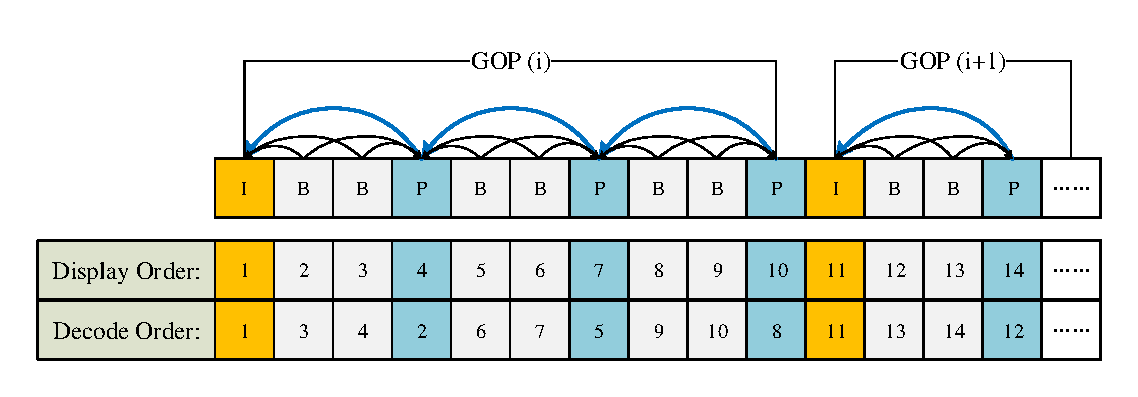
\includegraphics[width=0.45\textwidth]{photo/H264_IPB.pdf}
\caption{A sample of GOPs in H.264}
\label{H264-IPB}
\end{figure}
\fi

\subsubsection{Video Frame Recovery}
In the circumstance of video approximate storage, it's common to lose some frames and leave the video incomplete. However, the lost frames may still be recoverable with the benefit of nowadays powerful deep learning techniques. One of them is named video frame interpolation [CITE][CITE].

Video frame interpolation is one of the basic video processing techniques, an attempt to synthetically produce one or more intermediate video frames from existing ones.This is a technique that can model natural motion within a video, and generate frames according to this modelling.

In deep learning methods, optical changes between the frames are trained in a supervised setup mapping two frames to their ground truth optical flow. Among all these, a multi-scale network\cite{van2017frame} based on recent advances in spatial transformers and composite perceptual losses as well as a context-aware Synthesis approach\cite{niklaus2018context} have so far produced the new state-of-the-art results in terms of PSNR and middlebury benchmark respectively.


\subsection{Existing Erasure Codes}\label{existEC}
Reliability is a critical issue since disk failures are typical in storage systems. To improve the reliability of storage systems, several RAID forms (e.g., RAID-5, RAID-6, 3DFTs) and erasure codes are proposed by researchers.  Traditional erasure codes can be categorized into two classes, Maximum Distance Separable (MDS) codes and non-MDS codes. MDS codes aim to offer data protection with optimal storage efficiency. On the other hand, non-MDS codes improve the performance or reliability by consuming extra storage space.

In the past two decades, several
famous erasure codes are proposed for double Disk Failure Tolerant arrays (2DFTs or RAID-6), such as EVENODD code [CITE], RDP code [CITE], Blaum-Roth code[CITE], X-code [CITE], Liberation code [CITE], Liber8tion code [CITE], Cyclic [CITE] code, B-Code [CITE], Code-M [CITE], H-code [CITE], P-code [CITE] and HVcode [CITE], etc.

In Triple Disks Failure Tolerant Arrays (3DFTs), typical MDS codes include Reed-Solomon codes [CITE], Cauchy-RS codes [CITE], STAR code [CITE], Triple-Star code [CITE], Triple-Parity code [CITE], HDD1 code [CITE], RSL-code [CITE], RL-code [CITE], and so on. Typical non-MDS codes contain WEAVER codes [CITE], HoVer
codes [CITE], T-code [CITE], HDD2 code [CITE], Pyramid codes [CITE], Local Reconstruction Codes [CITE], Locally Repairable Codes [CITE], etc.

Several classic erasure codes are illustrated in detail as below,

%从这里开始简单讲解几种RAID-6或三盘容错阵列的纠删码,如RS,EVENODD,RDP,STAR,LRC, H-Code,TIP-Code等,并且用编码图来说明(主要是实验中用到的几种编码)。

\subsection{Approximate Storage}
%Storage techniques nowadays generally regard all information of the same importance, which causes significant costs in energy, disk drives and computing resources. But not all data need high-reliability storage for its backup. That is why the concept of approximate storage is introduced. 
Approximate Storage is another way outside of traditional methods of trading off the limited resource budget with the costly reliability requirements, which recently receives more attentions since data centers are faced with storage pressure from the ever-increasing data.

Use cases for approximate storage range from transient memory to embedded settings and mass storage cloud servers. Mapping approximate data onto blocks that have exhausted their hardware error correction resources, for example, to extend memory endurance. On embedded settings, it enables the reduction of the cost of accesses and preserve battery life to loosen the capacity constraints. \cite{sampson2014approximate} Here, in data-center-scale video database, approximate storage can provide multiple levels of fault tolerance for data of different importance, avoiding redundant backup for the less-important data, thus saving a significant amount of space.


Approximate storage loosens the requirement of storage reliability by allowing quality loss of some specific data. Therefore, programmers can specify the importance of the data segments and assign them to different storage blocks. The critical data is still safe because they are stored and sufficiently backed up by expensive and highly reliable storage devices. Meanwhile, non-critical data is exposed to error, thus increasing storage density and saving cost.

%However, it is too naive to store data in approximate storage units indiscriminately. Related research \cite{guo2016high} shows that this can lead to unacceptable data pollution. To ensure data quality in this case, higher error correction costs are required resulting in an increase in overall storage costs. Therefore, it is very important to distinguish the importance of video data. 

\begin{table}[ht]
\centering 
\caption{Comparison of storage overhead, reliability and performance between EC, Approximate Storage and Approximate Code. (``Appr.'' is short for ``Approximate'')}\label{tab-AS-EC-AP}
\begin{tabular}{|c|c|c|c|c|}
\hline
\multicolumn{2}{|c|}{Schemes} & \begin{tabular}[c]{@{}c@{}}Storage\\ Overhead\end{tabular} & Reliability & Performance \\ \hline
\multirow{2}{*}{EC} & RS & high & high & medium \\ \cline{2-5} 
 & RAID-6 & medium & medium & high \\ \hline
\multicolumn{2}{|c|}{Appr. Storage} & low & low & high \\ \hline
\multirow{2}{*}{\begin{tabular}[c]{@{}c@{}}Appr.\\ Code\end{tabular}} & ID & \multirow{2}{*}{low} & high & high \\ \cline{2-2} \cline{4-5} 
 & UD &  & medium & high \\ \hline
\end{tabular}
\end{table}

\subsection{Our Motivation}
Based on Table \ref{tab-AS-EC-AP}, either the existing erasure codes or the approximate storage methods cannot meet the requirements of video applications in the cloud storage system due to the following reasons. 

First, the overhead of existing 3DFTs erasure codes is too high.
Second, the 2DFTs erasure codes sacrifice part of reliability, and the reliability of approximate storage schemes are much lower since they cannot tolerate disk-level failures.
Finally, existing erasure codes provide the same fault tolerance for all data without distinction, resulting in the same reliability for error-sensitive data and robust data.

Based on these reasons, we propose a scheme for tiered video storage in a highly reliable environment, Approximate Code.
Approximate code is an erasure code framework that uses tiered storage\cite{krish2014hats} \cite{wang2014balancing} \cite{zhang2010automated} \cite{udipi2012lot} and approximate storage strategies to separate an existing erasure codes into codes with different fault tolerances and apply them to important and unimportant data.

\begin{figure*}[ht!]
\centering
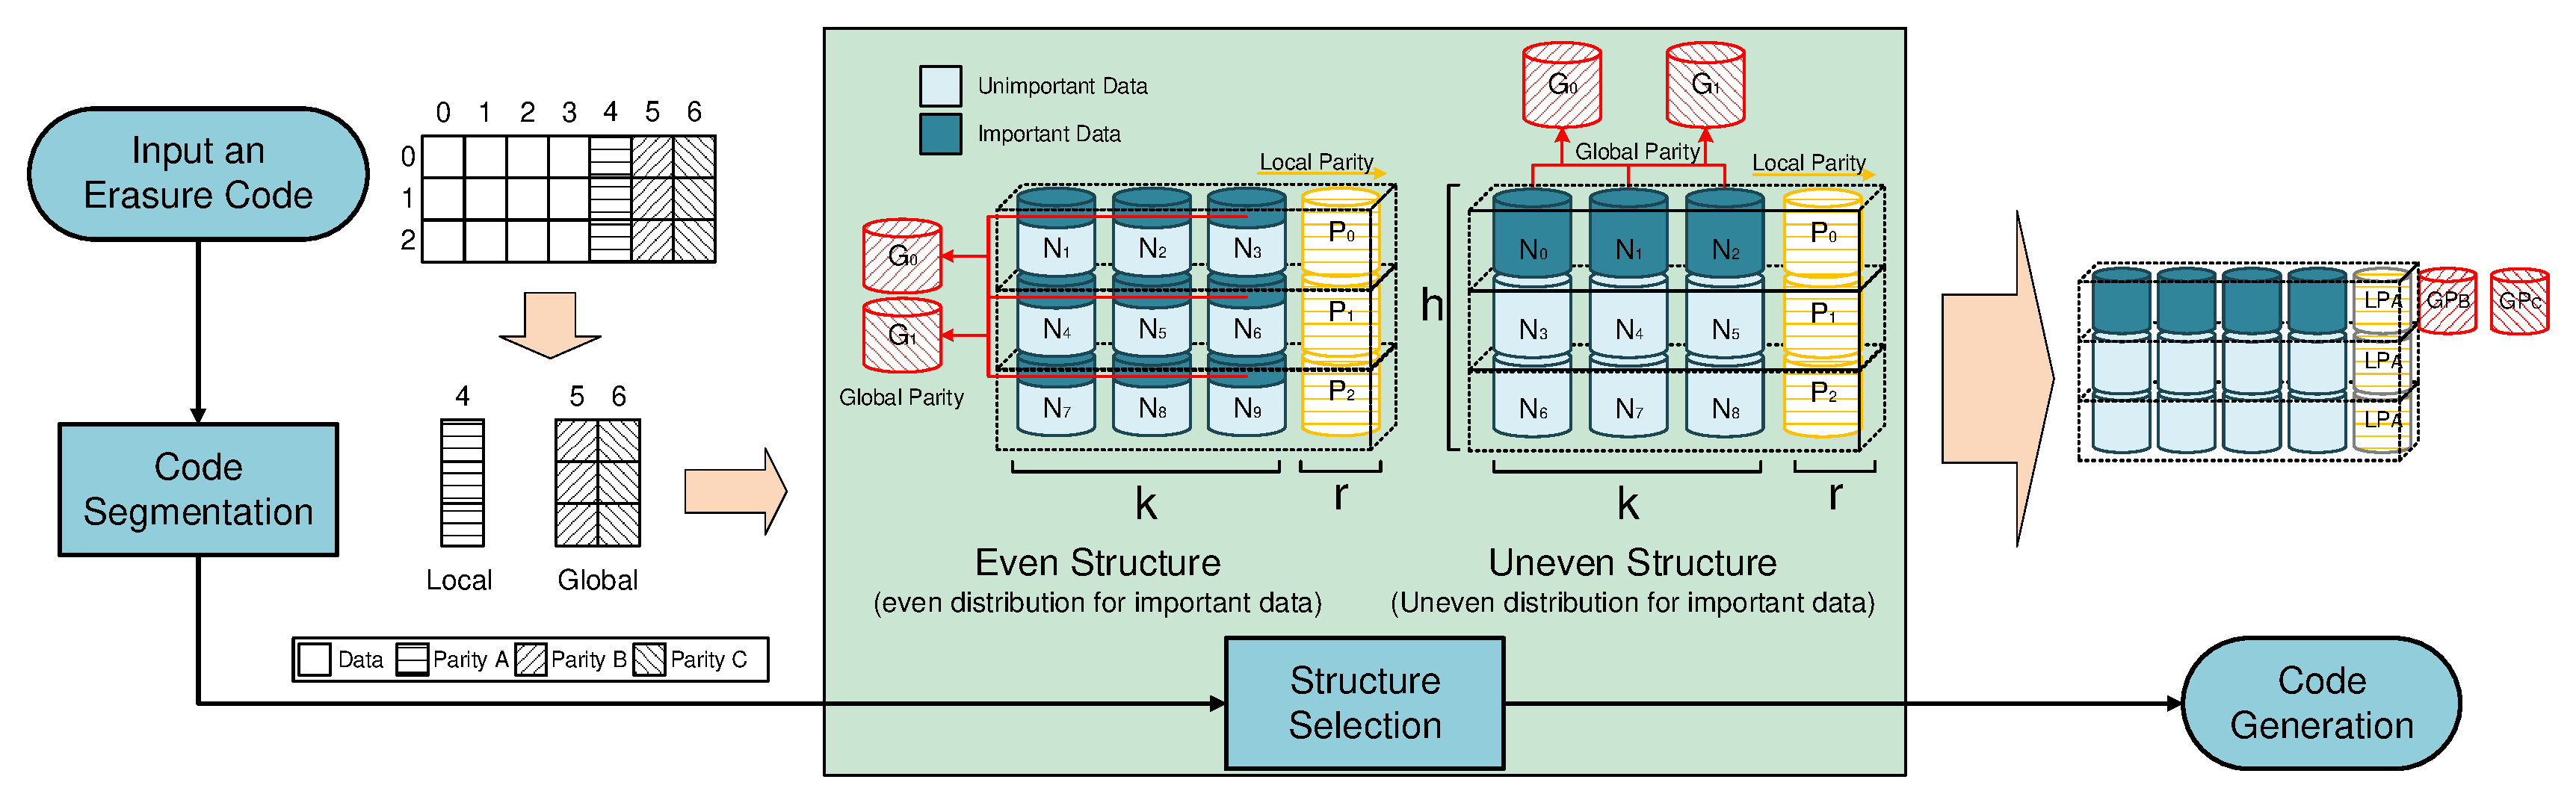
\includegraphics[width=\linewidth]{photo/Framework-v2.pdf}
\caption{The framework of Approximate Code}
\label{fig-framework}
\end{figure*}

\section{Approximate Code}\label{ApCode}
In this section, we introduce the Approximate Code Framework and its properties through a few simple examples. 

\subsection{Overview of Approximate Code Framework}
The Approximate Code mainly includes three operations: code segmentation, structure selection and code generation. We use Figure \ref{fig-framework} to illustrate our design.

\subsubsection{Code Segmentation}
For an input erasure code, we assume that its fault tolerance is $x$. The Approximate Code first splits its parity block into two parts: local and global. The former verifies all important and non-critical data, while the latter only verifies important data. Code segmentation are designed to ensure that local parities can tolerate any $r$ node failures, so the fault tolerance of non-critical data is $r$. For important data, the code segmentation ensures that the parity block of important data can be completely recombined into the original $x$DFTs erasure code scheme. 

In the example, a 3DFTs erasure code with 4 data chunks and 3 parity chunks is input, and its 3 parity chunks are separated into two local and one global parity chunks.

\subsubsection{Structure Selection}
The Approximate Code framework then choose the structure for the input erasure code.
There are two main structures that distribute important and unimportant data in different ways.
As shown in Figure \ref{fig-framework}, in \emph{Structure I}, important data occupies 1 block in each node, and in \emph{Structure II}, it occupies 1 data arrays.
We specify that in \emph{Structure I}, the ratio of important data to each node is $1/h$, thereby ensuring that the number of important data in both \emph{Structure I} and \emph{Structure II} just fills up $k$ nodes.

Since \emph{Structure I} distributes important data across each node, it guarantees a more balanced load. \emph{Structure II} concentrates important data into an array, and provides greater reliability for important data. A detailed analysis of this will be presented in \ref{evaluation}.

\subsubsection{Code Generation}
After code segmentation and structure selection, the Approximate Code Framework generates an approximate form of the input erasure code.

The construction of the Approximate Code is determined by 5 parameters $k$, $r$, $g$, $h$ and $Structure$. 
We define the naming rules of the output Approximate Code as \textbf{``Approximate XXX Code ($k,r,g,h, Structure$)''}, where ``XXX'' is the name of input erasure code. Paremeter $Structure$ is I or II and it can be omitted when not focusing on the specific construction.

In a $n$-node array, $k$ of them are data nodes and $r=n-k$ nodes are for local parity, where each node can be divided into multiple blocks.
Approximate Code are designed for $h$ arrays, therefore it includes $k*h$ data nodes and $r*h$ local parity nodes.
Besides them, $g$ nodes are designed for global parity, which are calculated only by the important data blocks, so the total number of nodes in Approximate Code ($k,r,g,h$) is 
$h*(k+r) + g$.

Approximate Code guarantees that the unimportant data can tolerate any $r$ node failures and the important data can tolerate any $r+g$ node failures.
Since the 3DFTs is a tipical configuration, we mainly discuss the situation of $r+g=3$, so $r$ is usually set to 1 or 2.

\iffalse
\begin{figure}[]
\centering
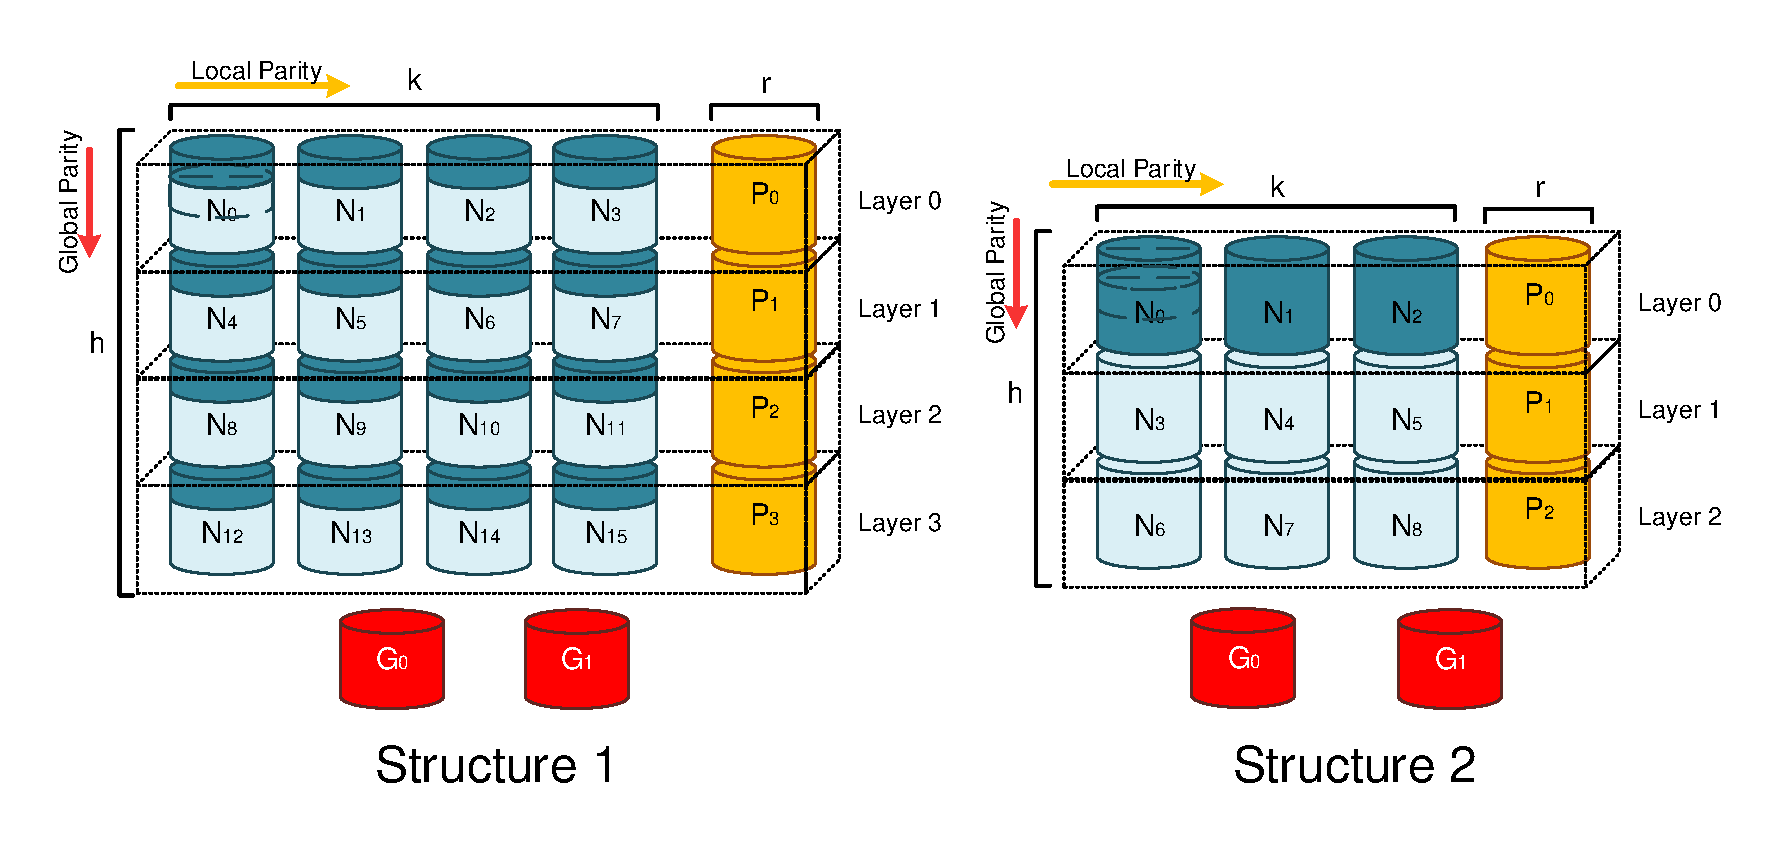
\includegraphics[width=\linewidth]{photo/AP-kmha-v7.pdf}
\caption{A sample of Approximate Codes $(4,1,4)$ in \emph{Structure I}, and Approximate Code $(3,1,3)$ in \emph{Structure II}.
Data nodes are marked as $N_i$, important data are marked as water green, local parity nodes are marked as orange and global parity nodes are marked as red.
}
\label{fig-ap-414}
\end{figure}

\begin{figure}[htb]
\centering
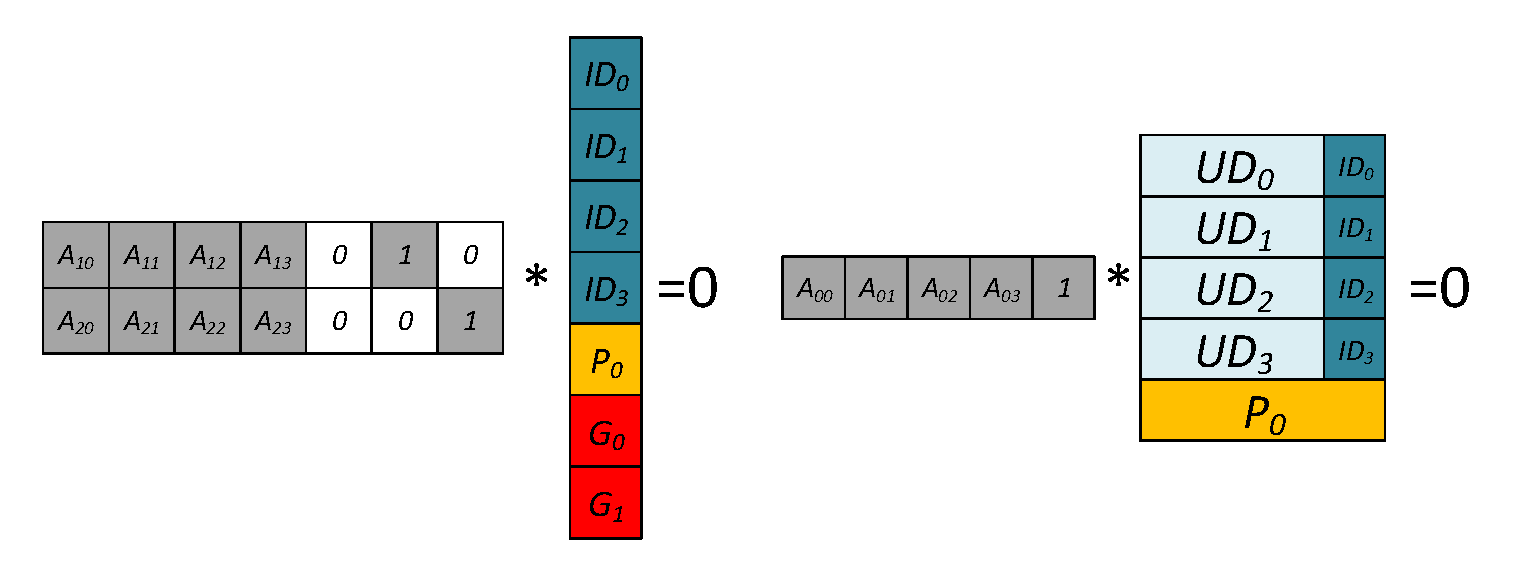
\includegraphics[width=0.45\textwidth]{photo/AP-RS-43.pdf}
\caption{The generate matrix of RS-based Approximate Codes $(4,1,4)$, where $ID_i$ and $UD_i$ represent the important and unimportant data in $N_i$. $G_0$ and $G_1$ are the parity blocks corresponding to important data blocks.}
\label{fig-ap-rs}
\end{figure}
\fi

\subsection{Approximate RS Code}
For RS(k,p), it can be seen that it provides $p$ independent horizontal parity nodes for $k$ data nodes. Therefore, the code segmentation for RS is arbitrary, that is, it supports any $r=p-g(0<g<p)$. RS also supports both two structures. 

For the situation shown in Figure \ref{fig-framework}, we consider the input erasure code as RS(4,3). It is divided into two local parities and one global parities with the \emph{Structure II} and it generate Approximate RS Code (4,2,1,3,II).
As a result, the unimportant data constitutes RS(4,2), and the important data constitutes RS(4,3).


\subsection{XOR-based Approximate Code}
Since we mainly provide 3DFTs for important data, we prefer to construct Approximate Code with several XOR-based codes to provide faster encoding and reconstruction speed than RS. This section introduce two tipical construction of XOR-based Approximate Code, Approximate STAR Code and Approximate TIP Code.


\begin{figure}[ht]
\centering
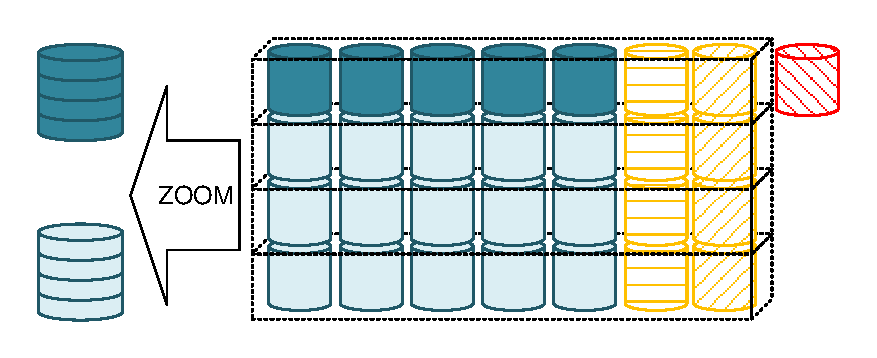
\includegraphics[width=0.8\linewidth]{photo/AP-5214.pdf}
\caption{Construction of Approximate STAR Code (5,2,1,4,II)}
\label{fig-ap-5214}
\end{figure}

\begin{figure}[ht]
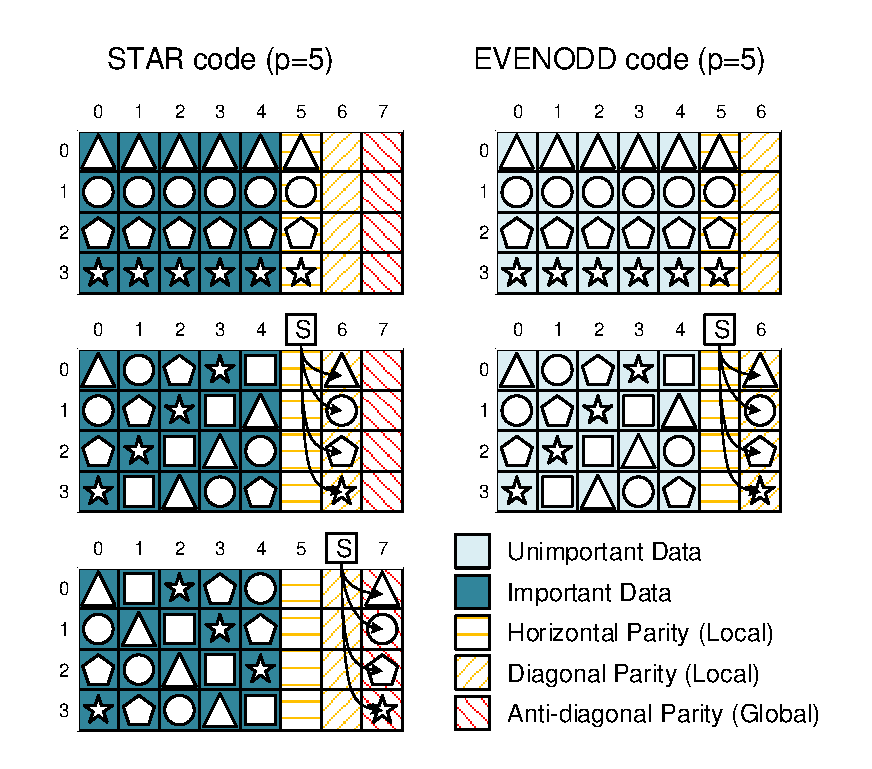
\includegraphics[width =0.8\linewidth]{photo/EVENODD-STAR-v2.pdf}
\caption{EVENODD only consist horizontal and diagonal parity, while STAR add the anti-diagonal parity node based on EVENODD and can tolerate 3 device failures.}\label{fig-star}
\end{figure}

\subsubsection{Approximate STAR Code}
Figure \ref{fig-ap-5214} shows the construction of Approximate STAR Code (5,2,1,4,II).

As introduced in \ref{existEC}, STAR Code \cite{huang2008star} has 3 parity chunks and it is a tipical 3DFTs XOR-based erasure code.
%We usually split the XOR-based code into a horizontal parity (local) and (anti-)diagonal parities (global), whereas the STAR feature allows it to support another segmentation method.
Since STAR is a direct extension of EVENODD\cite{blaum1995evenodd}, that is to say, the STAR that removes the anti-diagonal parity is the typical RAID-6 code EVENODD. As shown in Figure \ref{fig-star}, in this case, the horizontal and diagonal parity are used as local parities while the anti-diagonal parity is defined as global parity.
According to the construction requirements of STAR, each node is divided into 4 blocks.

Briefly, Approximate STAR Code (5,2,1,4,II) can be thought of as important data encoded by the full STAR, while unimportant data is encoded by a part of STAR, EVENODD. It is plain to see that important data can tolerate any 3 node failures while unimportant data can tolerate any 2 node failures.

\subsubsection{Approximate TIP Code}

optimal update complexity.

Figure \ref{fig-ap-TIP} is a tipical construction of Approximate Code ($5,1,6$) in \emph{Structure I}, based on RAID5 and TIP-code \cite{zhang2015tip}. RAID5 tolerate one node failure while TIP-code is an XOR-based 3DFTs code. In each array, local parity blocks provide horizontal XOR parity, and between arrays, global parity provide diagonal parity and anti-diagonal parity. 

The local (horizontal) parity elements are calculated by the following encoding equations.
\begin{align}
    LP_{i,0} &= \bigoplus_{j=0}^{k-1} ID_{i,j} (0 \leqslant i < h)\\
    LP_{i,p}(0<p<s) &= \bigoplus_{j=k(p-1)}^{kp-1} UD_{i,j} (0 \leqslant i < h)
\end{align}

When generating global parity blocks, the important data block, the local parity block, and the global parity block should be arranged as the encoding form of TIP-code. Figure \ref{fig-TIP} shows the coding method of diagonal and anti-diagonal parity blocks.
Since the encoding process of important data blocks can be seen as RAID5 plus TIP-code, it is obvious that they achieve 3DFTs.

\begin{figure}[ht]
\centering
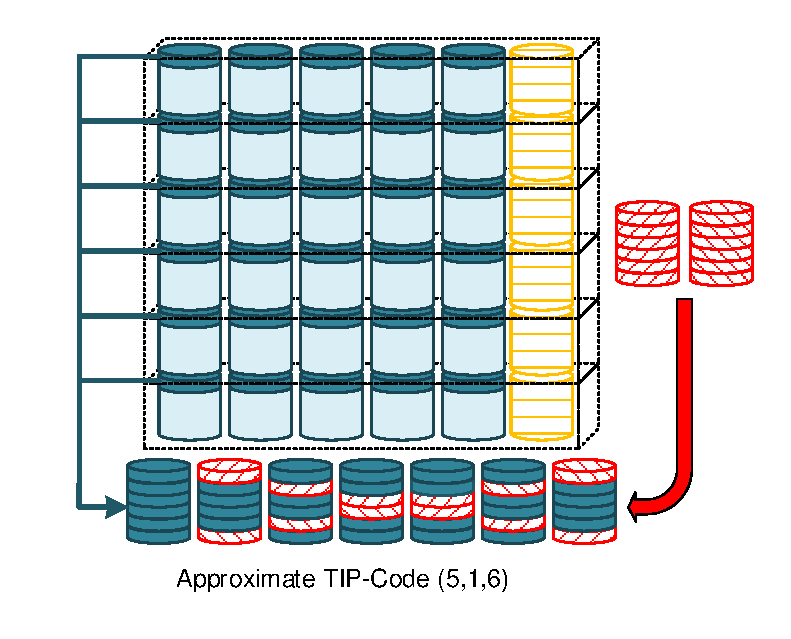
\includegraphics[width=0.3\textwidth]{photo/AP-516.pdf}
\caption{The XOR-based Approximate Code ($5,1,6$, \emph{Structure I}), constructed based on RAID5 and TIP-code.}
\label{fig-ap-TIP}
\end{figure}

\begin{figure}[ht]
\subfigure[]{
\begin{minipage}[t]{0.45\linewidth}
\centering
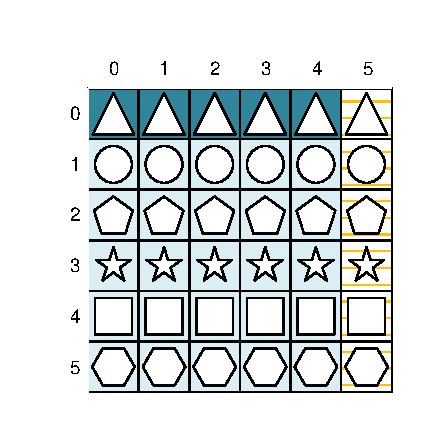
\includegraphics[width=0.8\linewidth]{photo/RAID5.pdf}        
\end{minipage}
}
\subfigure[]{
\begin{minipage}[t]{0.45\linewidth}
\centering
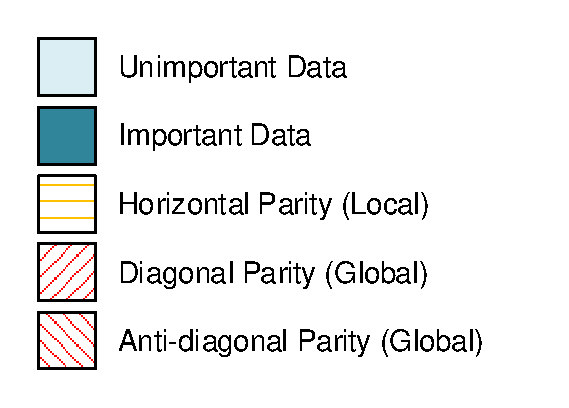
\includegraphics[width=0.8\linewidth]{photo/legend.pdf}        
\end{minipage}
}

\subfigure[]{
\begin{minipage}[t]{0.45\linewidth}
\centering
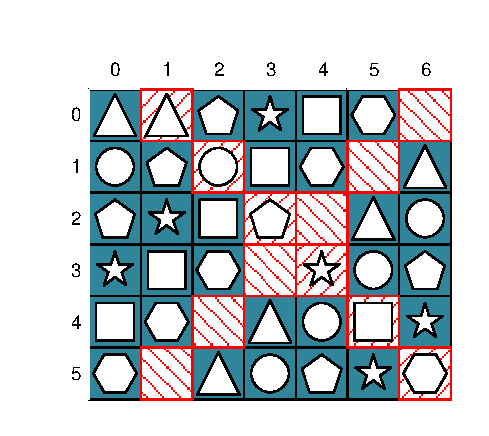
\includegraphics[width=\linewidth]{photo/TIP-di.pdf}        
\end{minipage}
}
\subfigure[]{
\begin{minipage}[t]{0.45\linewidth}
\centering
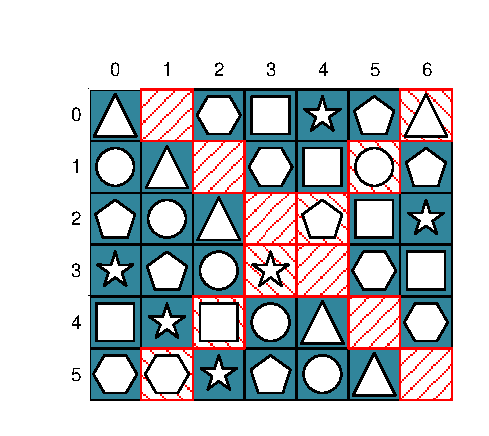
\includegraphics[width=\linewidth]{photo/TIP-an.pdf}        
\end{minipage}
}
\caption{Encoding pf TIP-code}
\label{fig-TIP}
\end{figure}

\iffalse
\subsection{Case Study}
This section describe the decoding methods in different cases of node failure based on \emph{Structure I} and \emph{Structure II}.

\subsubsection{Reconstruction cases in Structure 1}
Under \emph{Structure I}, important data and unimportant data are distributed in the same nodes, so they suffer the same risk of device failures. 
When $r$ or less nodes fail, all the data can be reconstructed by local parity.
When the number of failed nodes is over $r$ but no more than 3, the Approximate Code conduct approximate recovery, in which the important data are recovered by global parity nodes and the damaged video data will be processed by the video recovery and fuzzy algorithm.

\subsubsection{Reconstruction cases in Structure 2}
Under \emph{Structure II}, we consider important and unimportant data nodes separately.

For node level failure, the fault tolerance of \emph{Structure II} is exactly as \emph{Structure I},When it comes to node level failures, \emph{Structure II} can tolerate more unimportant data node failures than \emph{Structure I}. The parity chain of important data does not pass through the unimportant data, so the damage of these nodes does not affect the recovery of important data.

///////////////////////
Under the random probability model of nodes, the probability of failure of the Approximate Code under 4 node damage is
\begin{equation}
    P_{failure} = \frac{C_{k+3}^4}{C_{(k+r)h+3-r}^4}
\end{equation}
which is the 4 node failure situation in $k$ important data nodes and 3 important parity nodes. For example, the failure situation of Approximate Code ($4,1,4$, \emph{Structure II}) probability is 0.478\%.
\fi

\subsection{Properties of Approximate Code}\label{properties}

We analyze the nature of the Approximate Code from the following aspects, and the calculation method of the relevant indicators is given in Table \ref{tab-AS-RS-AP}.
\begin{itemize}
    \item Low Storage Overhead: Approximate Code reduces storage overhead by approximating storage strategies. This property is more pronounced for data with a smaller proportion of important data.
    \item Low Update Overhead: When one node is updated, Approximate Code only needs to write $r \times h$ local parity nodes and only $3-r$ global parity nodes, while tipical 3DFTs EC methods should write $3 \times h$ parity nodes.
    \item High reliability for important data. The Approximate Code guarantees 3DFTs for important data.
    \item Flexibility. The implementation of the Approximate Code can be based on RS, XOR or a mixture of the two.
\end{itemize}

\begin{table}[]
\centering 
\caption{Comparison of storage overhead and fault tolerance between Ap-Code (short for Approximate Code), RS and several XOR-based codes.}\label{tab-AS-RS-AP}
\begin{tabular}{|c|c|c|c|}
\hline
EC & \begin{tabular}[]{@{}c@{}}Storage\\ Overhead\end{tabular} & \begin{tabular}[]{@{}c@{}}Fault \\ Tolerance\end{tabular} & \begin{tabular}[]{@{}c@{}}Single Node\\Update Cost\end{tabular} \\ \hline
RS($k,q$) & $(k+q)/k$ & $q$ & q \\ \hline
EVENODD($k,2$) & $(k+2)/k$ & 2 & 2 \\ \hline
TIP-code/STAR($k,3$) & $(k+r)/k$ & 3 & 3 \\ \hline
\begin{tabular}[]{@{}c@{}}Ap-Code\\ ($k,r,h$)\end{tabular} & $\frac {(k+r)h+3-r}{k \times h}$ & r to 3 & $r+\frac{3-r}{h}$ \\ \hline
\end{tabular}
\end{table}

\subsection{Implementation}\label{Implementation}
\begin{figure}[htb]
\centering
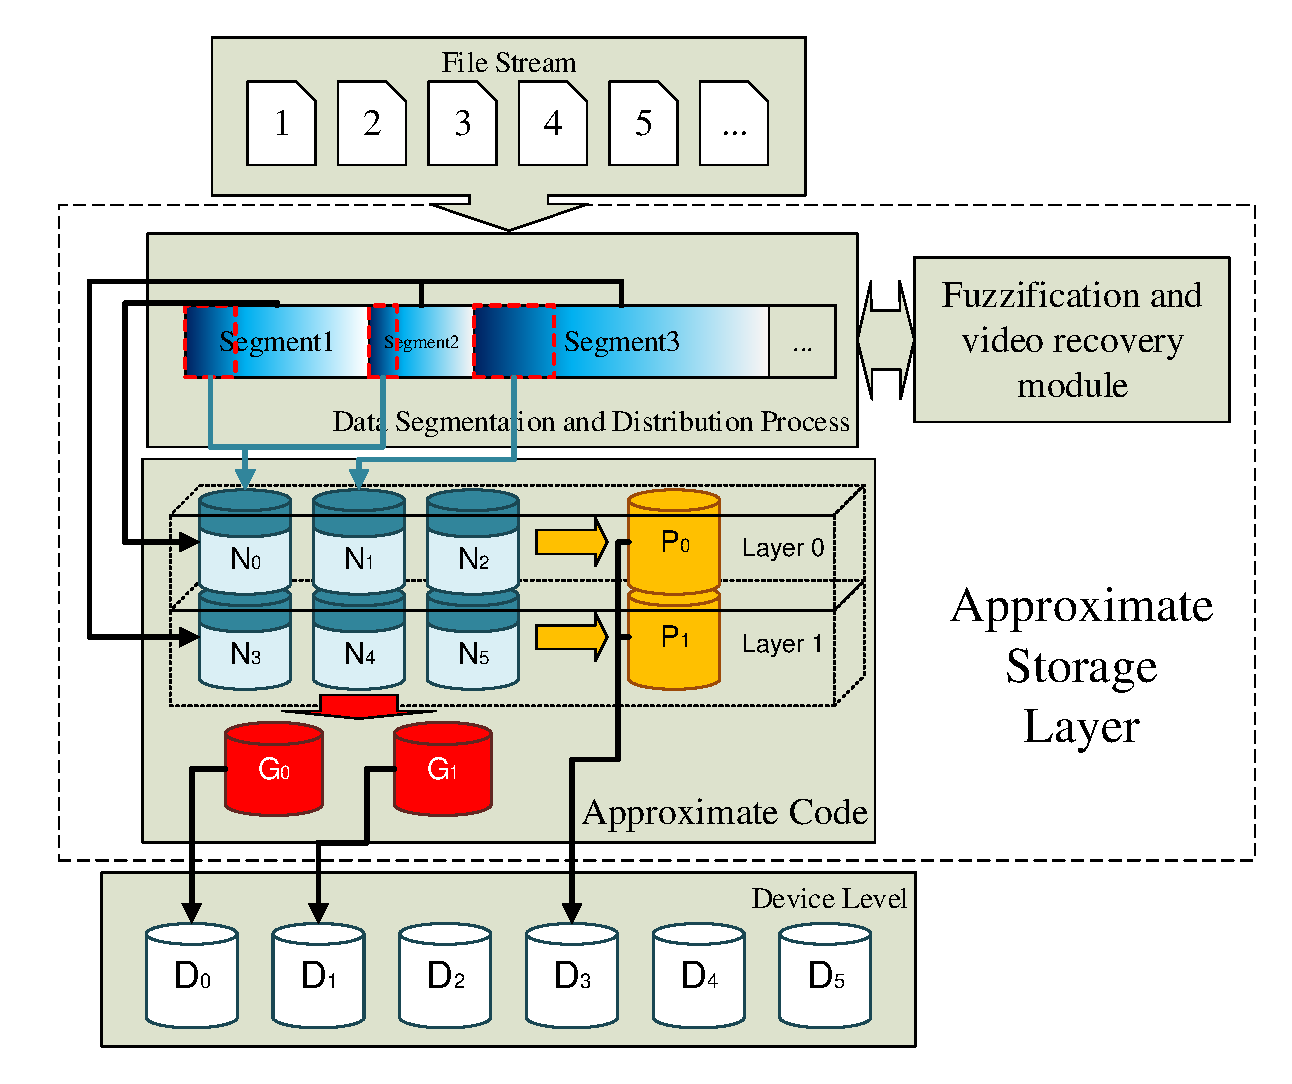
\includegraphics[height = 5cm]{photo/implementation-V2.pdf}
\caption{Overview of Approximate Code implementation}
\label{fig-implementation}
\end{figure}

Compared with the traditional scheme that does not consider the meaning of the upper array data, the Approximate Code pays attention to the difference of the importance of the data, so an intermediate array between the upper array application and the underlying distributed storage system is necessary to preprocess the data. We call it the approximate storage array, which include 3 parts: data identification and allocation, encoding and decoding process of Approximate Code and the video fuzzification and recovery.

\subsubsection{Data Segmentation and Distribution module}
The data segmentation module splits the video file stream into multiple data segments and automatically discriminates the important data. A natural approach is to follow the GOP segmentation. According to the \ref{video storage}, the GOP of the encoded video starts with an I frame, and all the data in that GOP depends on it for decoding, so we define it as important data and divide the GOP into I frames (important part) and other data. (unimportant part).

The data distribution module distributes important data and unimportant data in different blocks and records the location. This location information is also defined as important data. This module is also responsible for analyzing the proportion of important data and unimportant data in the data stream to select the most appropriate coding parameter configuration to ensure fault tolerance and high storage efficiency of important data.

\subsubsection{Approximate Code module}
The Approximate Code module is responsible for encoding and decoding important and unimportant data and completely recovering the data within fault tolerance. For data that cannot be recovered, the Approximate Code module transmits it to the video recovery module for approximate recover videos.

Approximate Code module is also responsible for allocating blocks of data to ensure that blocks of each array are distributed to different nodes, while ensuring that global check blocks and data blocks are not on one node.

\subsubsection{Data Fuzzification and Video Recovery}
In the approximate recovery mode, the remaining data and important data are transferred to this module. Using a series of methods described in Section \ref{video storage}, frames that suffer from frame loss will be recovered using the interpolation algorithm; the corrupted frames will be processed into fuzzy images and approximately recovered by superpixel techniques.

\iffalse
\section{Approximate Recovery}\label{ap-recovery}
\begin{figure*}\label{fig-node-lost}
\subfigure{
    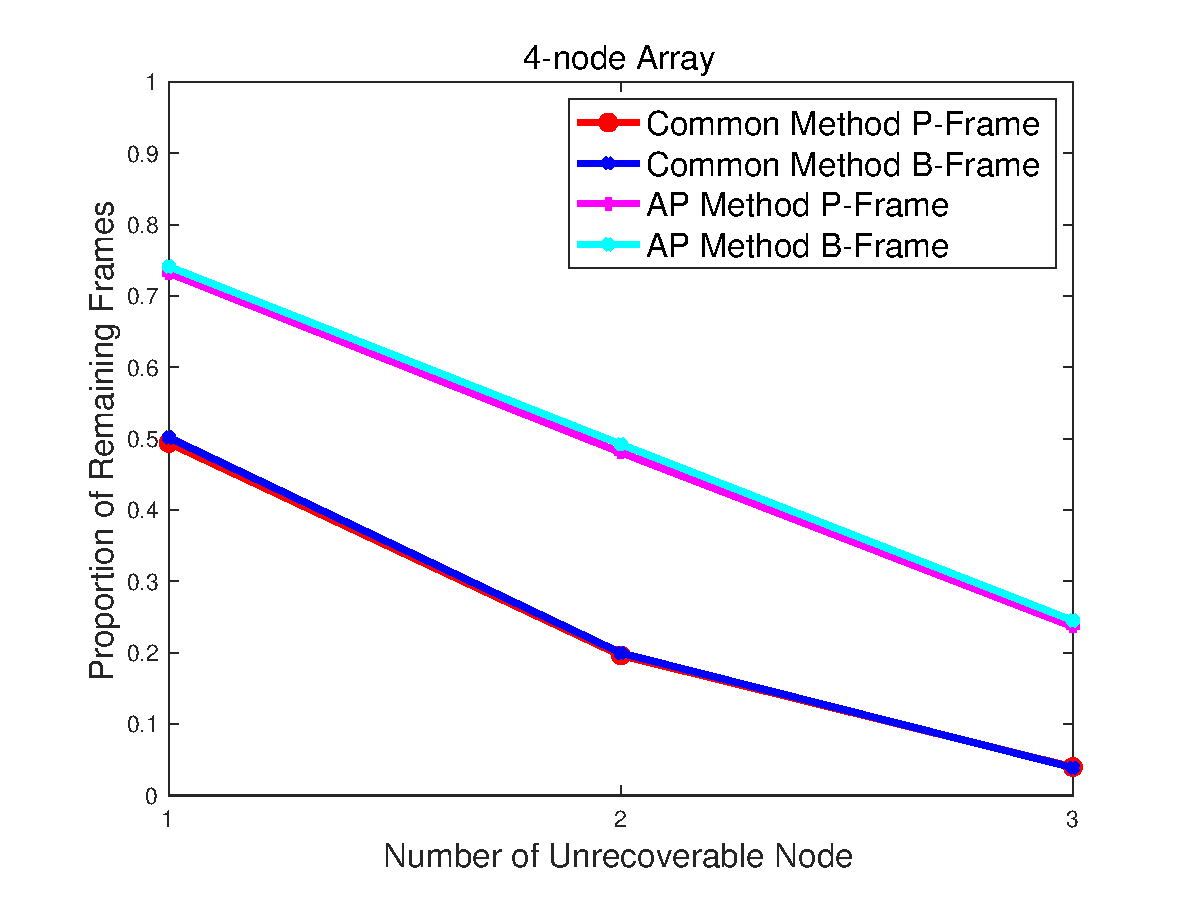
\includegraphics[width = 0.22\linewidth]{photo/experiment/Ap-recovery-4-disks.eps}
}
\subfigure{
    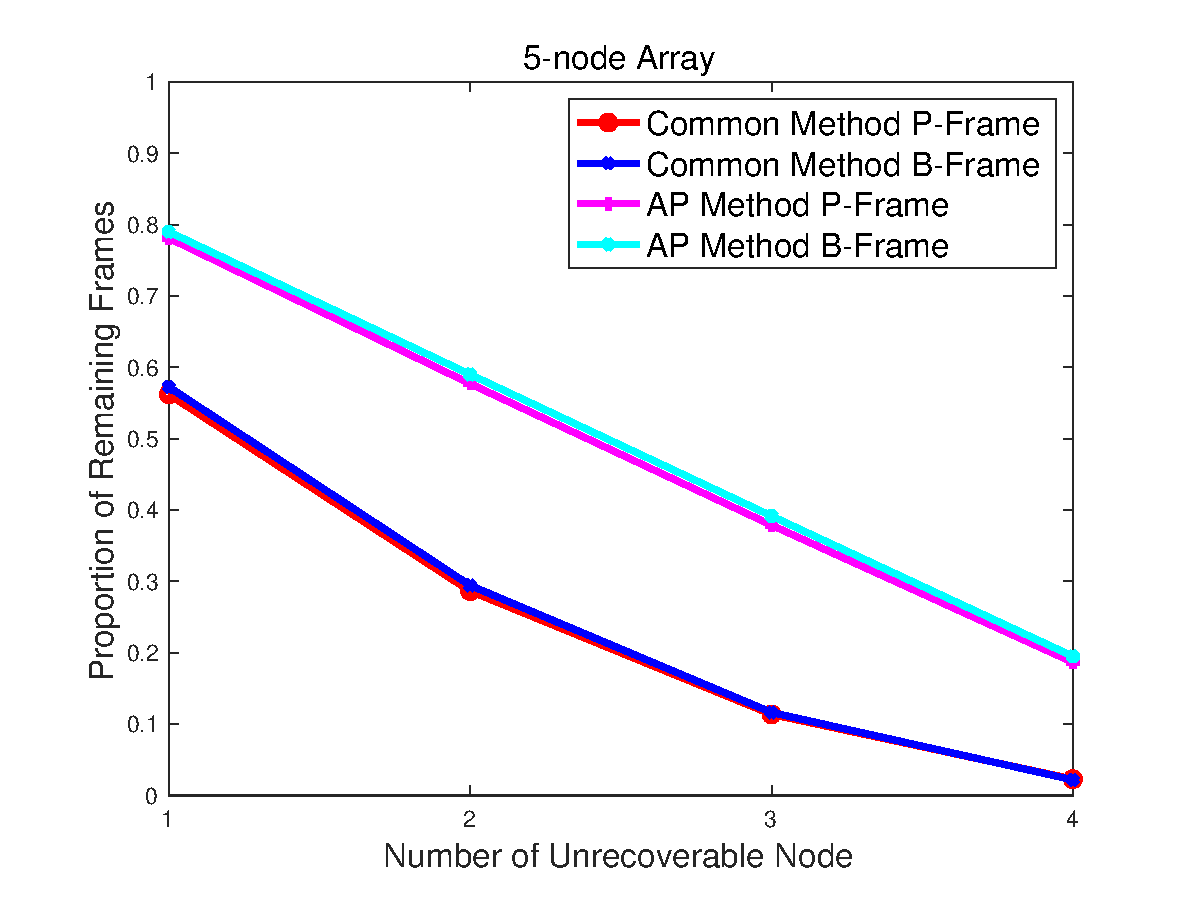
\includegraphics[width = 0.22\linewidth]{photo/experiment/Ap-recovery-5-disks.eps}
}
\subfigure{
    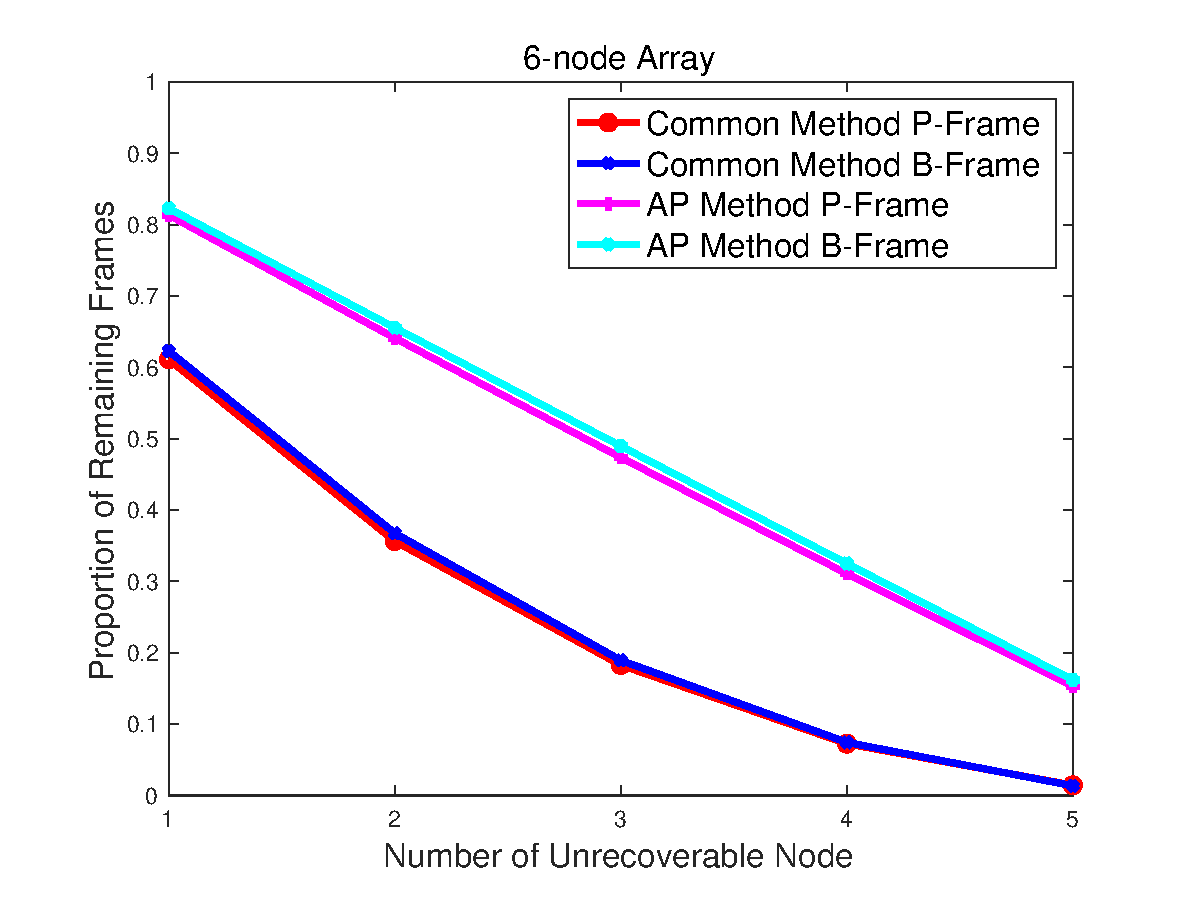
\includegraphics[width = 0.22\linewidth]{photo/experiment/Ap-recovery-6-disks.eps}
}
\subfigure{
    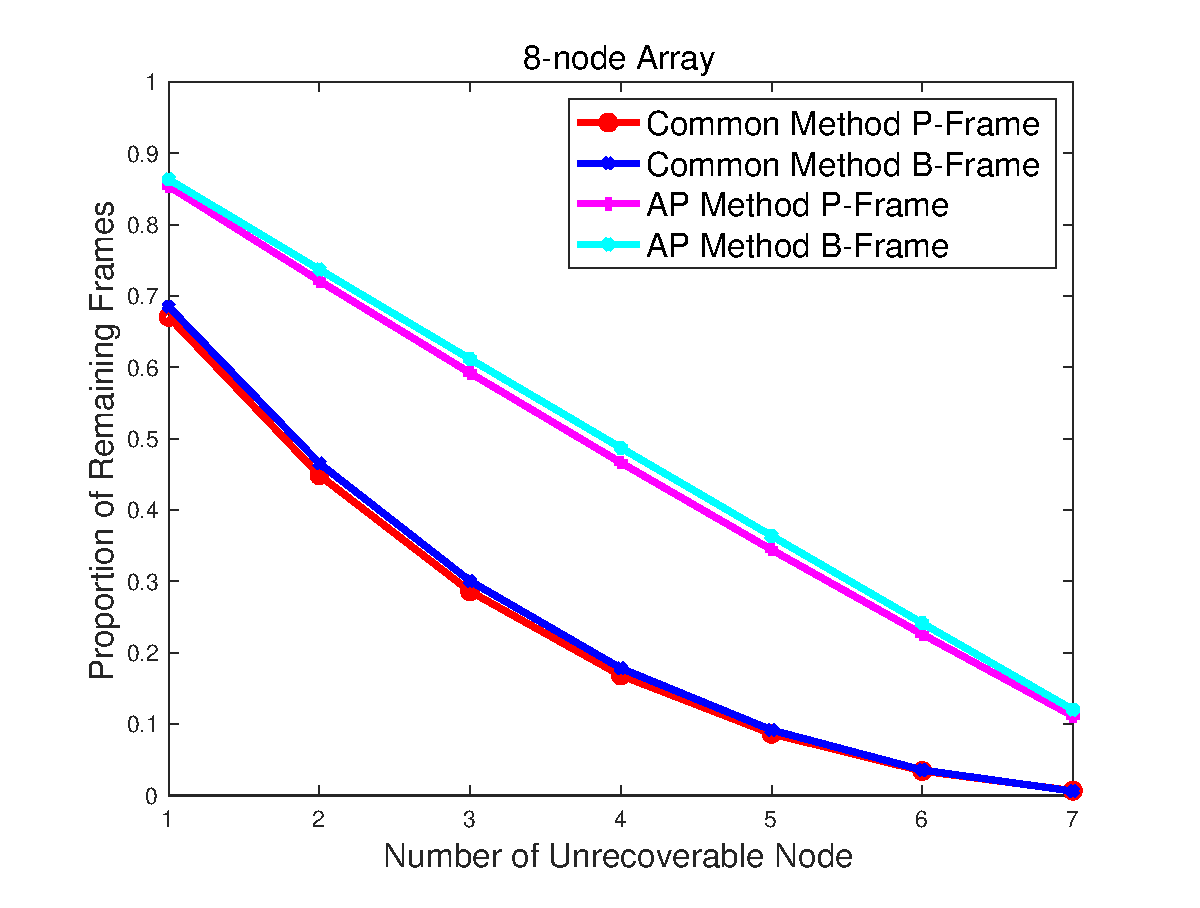
\includegraphics[width = 0.22\linewidth]{photo/experiment/Ap-recovery-8-disks.eps}
}
\caption{Comparison of the data retention  between approximate storage and common methods when node is unrecoverable.}\label{fig-node-lost}
\end{figure*}

In the approximate recovery mode, since unimportant data suffers unrecoverable loss, the recovery of damaged video files must be considered. Therefore, we evaluate the recovery of the video file in this section.

\subsection{Experimental Setup}
\subsubsection{Coding Algorithm} 
We evaluate the condition of the video of H.264 encoding [] under approximate recovery. Mainly because H.264 is an advanced video coding algorithm widely used at present, at the same time, the common advanced coding algorithms have similar coding processes.

\subsubsection{Data Set}
We choose 100 videos from xxx data set[]. All videos are stored in ``.mp4'' format at 1280*720 HD resolution.

\subsubsection{Metrics}
We use the number of frames saved as an indicator to evaluate the ability of the approximate storage and normal scheme to preserve data in the event of an unrecoverable node failure.

We define that when the I frame of the video is corrupted, the entire GOP is marked as unavailable (lost).

Since the approximation code stores the I frame as important data, the integrity of the I frame is always guaranteed in our scheme.

\subsubsection{Simulation}
We store the video files on a single disk according to the approximate storage scheme and the common scheme, while traversing the damage of all the disks, from 1 to n-1, and counting the number of damaged p-frames and b-frames. We use this to get the number of P and B frames that can be completely saved in the case of m out of n disks.

\subsection{Results}
The experimental results are shown in Figure \ref{fig-node-lost}, where $n$ is 4,5,6 and 8. In a 8-node array, when 2 nodes are unrecoverable, the approximate recovery method protects nearly 1/4 P or B frames, while the common method lost more than half of these frames. In addition, the approximate storage scheme can guarantee the number of frames of the video close to the theoretical limit.

\subsection{Analysis}
Our experiments prove that if data is stored indiscriminately, the loss of important data will seriously affect the security of all data, and our scheme will control the data loss near the theoretical limit, ensuring video recovery and fuzzification. feasibility.

\subsection{Frame Recovery ????}
\fi


\section{Evaluation}\label{evaluation}
In this section, we conduct a series of experiments to demonstrate the efficiency of Approximate Code in HDFS. 
\subsection{Evaluation Methodology }
We choose the RS code to compare with several XOR-based code, including TIP-code, EVENODD, STAR, RAID5 and RAID6. Since 3DFTs are typical configurations, we set the number of check nodes for the RS to 3.
Experiments as well as mathematical analysis are used to demonstrate the performance of Approximate Code.

\subsubsection{Metrics and Methods for Mathematical Analysis: }
We use the \textbf{Storage Efficiency}, \textbf{Fault Tolerance} and \textbf{Write(update) Cost} defined in Section \ref{properties} as measure.
We first analyze the impact of the settings of the three parameters on these metrics, then we compare these matrics with several EC methods.

\subsubsection{Metrics and Methods for Experiments: }
We use \textbf{Encoding Time} and \textbf{Recovery Time} as the metrics in our experiments.

Our experiment includes the calculation of these two metrics and can mainly be divided into several cases.
We measure the encoding time by calculating the time to generate all parity blocks, and we measure the recovery time by calculating the time to fully or approximately recover the failure nodes.
Both of them should be divided into 3 situation: single, double and triple node, so we discuss them separately.
Also, the encoding and recovery time consist of computation time, I/O time and transimission time in distributed file system, which should be considered separately.

The environment of our experiments are shown in Table \ref{tab-platform}. We set a Hadoop system with one NameNode and 4 DataNodes. \textcolor{gray}{text text text text text text text text text text text text text text text text text text text text text text text text text text text text text text text text text text text text text text text text text text text text text text text text text text text text text text text text text text text text text text text text text text text text text text text text text text text text text text text text text text text text text text text text text text text text text text text text text text text text text text text text text text text text text text text text }

\begin{table}[]
\begin{tabular}{|l|l|}
\hline
Description & DELL R730 Server \\ \hline
CPU & Intel Xeon 3.0GHz \\ \hline
NIC 1Gbps & 1Gbps \\ \hline
Memory & 32GB \\ \hline
Disk & 8TB HDD \\ \hline
OS & Linux 3.19 \\ \hline
Platform & Hadoop HDFS 3.0.3 \\ \hline
\end{tabular}
\caption{Details of Our Evaluation Platform}\label{tab-platform}
\end{table}

\subsection{Metrics and Methods of Experiment}
The metric of our experiments is time. The independent variable in this experiment is the number of nodes. We change the number of data nodes with different methods to compare the operation time. The experiments are divided into two parts, as one part is for measuring the encoding time of different methods, the other part is for timing the decoding time of different methods. The unit of the time is micro-second.\par

There are mainly two ways to compare different methods. One is for comparing the operational time of AP code with different parameters and that of one different method as we augment the number of data nodes. The other is for a general comparison with five data nodes for the encoding time, the decoding time in one disk, the decoding time in two disks and the decoding time in three disks for every method with its different parameters.\par

The environment of our experiment is listed below.


\subsection{Numerical Results of Mathematical Analysis}
\subsubsection{Encoding Time Analysis}
From the Figure xx a), we could find out that the AP code encodes largely faster than RS ($k$, $3$). The rate of optimisation between AP($k$, $1$, $6$) and RS ($k$, $3$) is from 976.4\% (3 nodes case) to 849.2\% (13 nodes case), as the encoding time of AP codes multiplies about 4.7 times and that of RS code multiplies about 4.2 times. The Figure xx b) and c) illustrate that the effet of Star code and Tip code is similar, and the difference between them and AP code is not very large. The rate of optimisation between AP ($k$, $1$, $6$) and Star ($k$, $3$) is from 125.6\% (3 nodes case) to 127.3\% (17 nodes case). According to Figure xx d), we could see that AP code largely reduces the encoding time, comparing to LRC method. The rate of optimisation between AP code (k, 1, 4) and LRC (4k, 2, 4) is from 596.0\% (3 nodes case) to 615.8\% (13 nodes case); and the rate of optimisation between AP code ($k$, $1$, $6$) and LRC ($6k$, $2$, $6$) is from 684.0\% to 443.1\%. Considering the optimisation rate, AP code ($k$, $1$, $4$) is the best among the four.\par



\begin{figure*}[]
\subfigure[AP and RS]{
    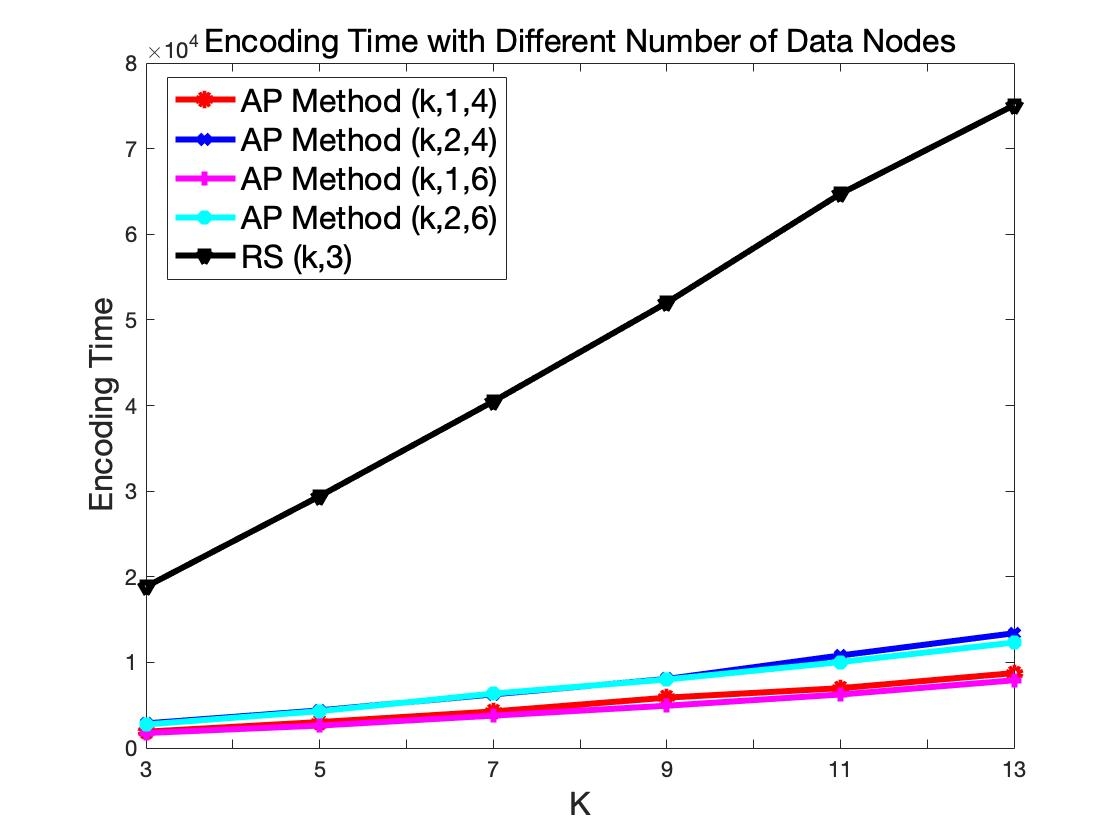
\includegraphics[width = 0.23\linewidth]{photo/experiment/Example1Modi2.jpg}
}
\subfigure[AP and STAR]{
    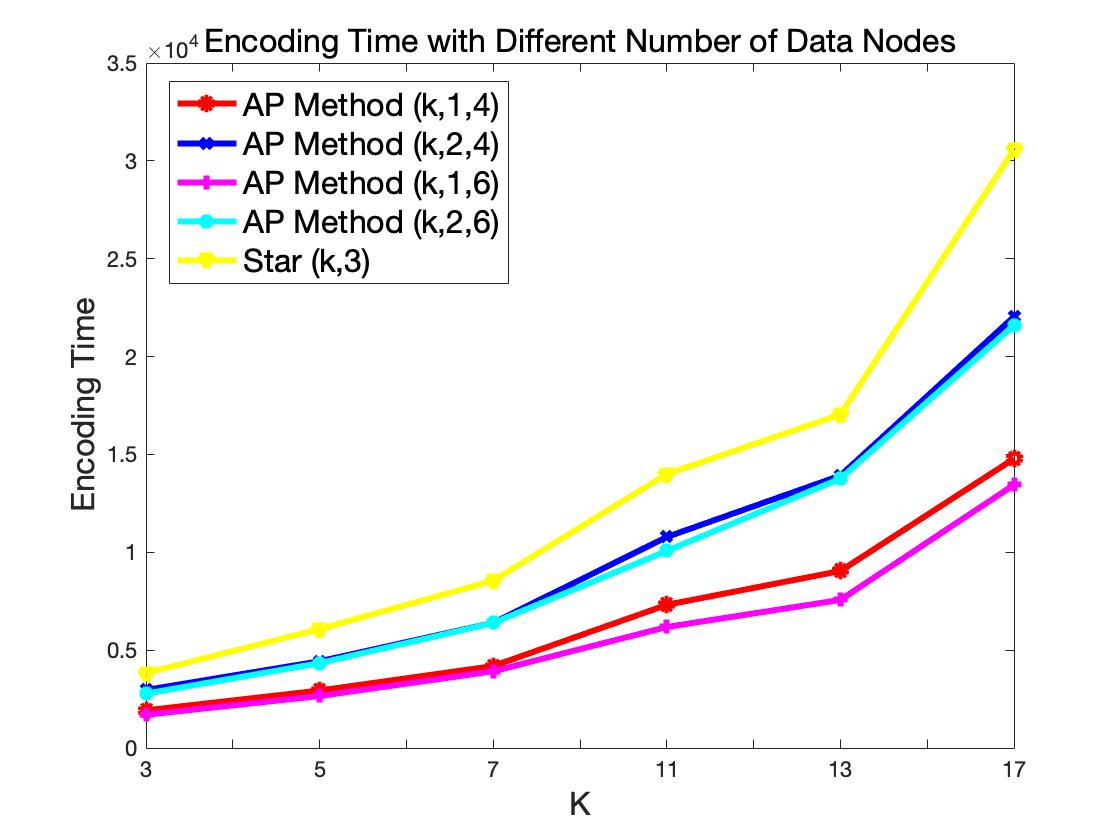
\includegraphics[width = 0.23\linewidth]{photo/experiment/Example2Modi1.jpg}
}
\subfigure[AP and TIP]{
    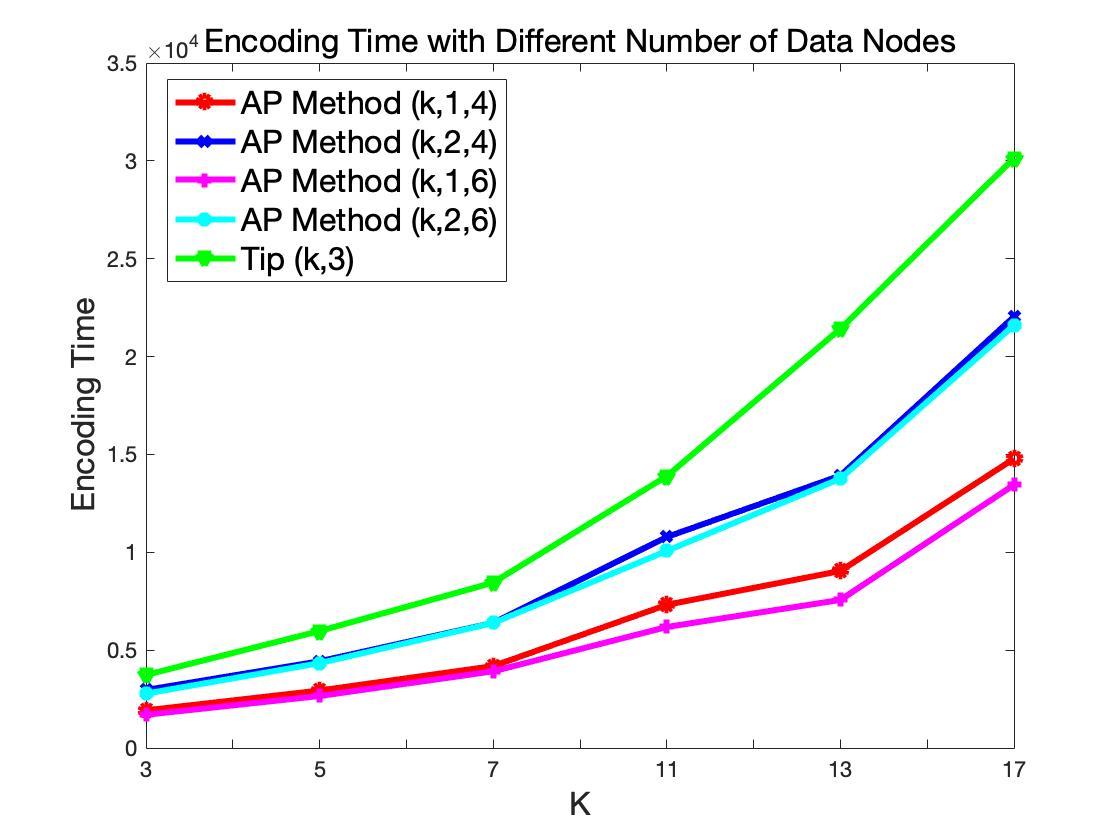
\includegraphics[width = 0.23\linewidth]{photo/experiment/Example3.jpg}
}
\subfigure[AP and LRC]{
    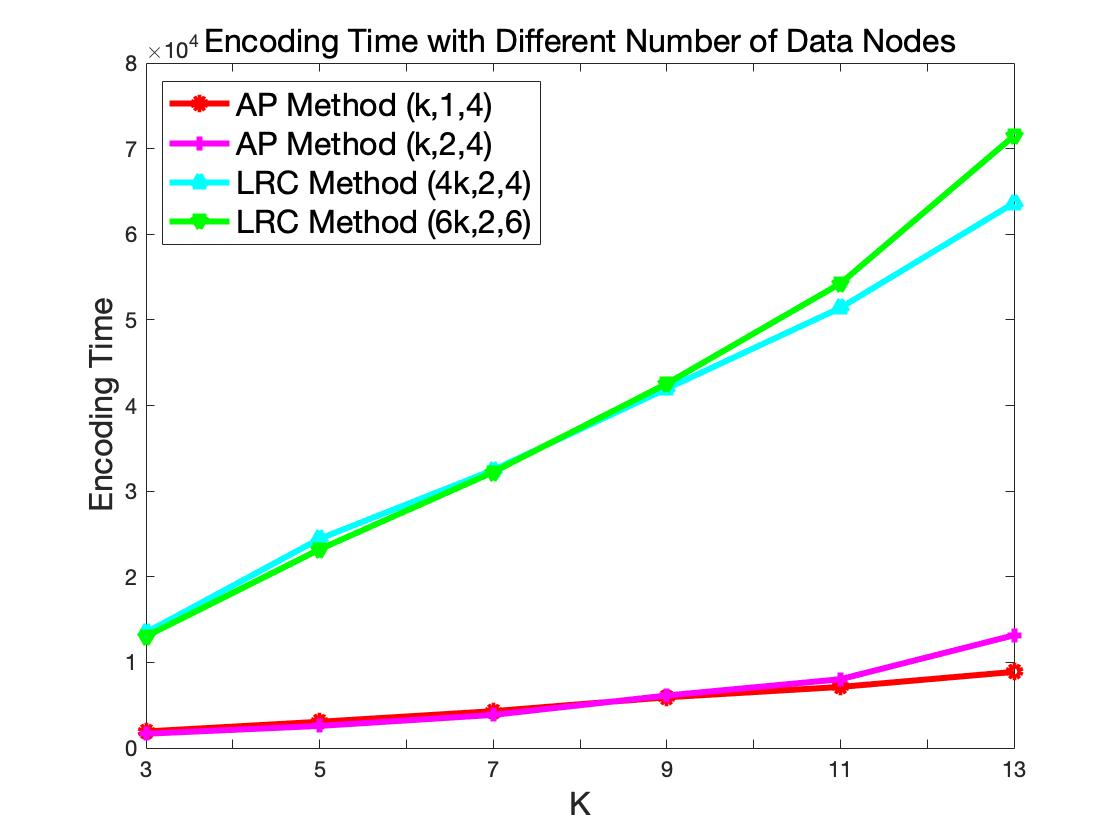
\includegraphics[width = 0.23\linewidth]{photo/experiment/Example4.jpg}
}
\caption{Encoding Time Comparison between AP method and other method}\label{fig-encoding}
\end{figure*}


\begin{figure*}[]
\subfigure[AP and RS]{
    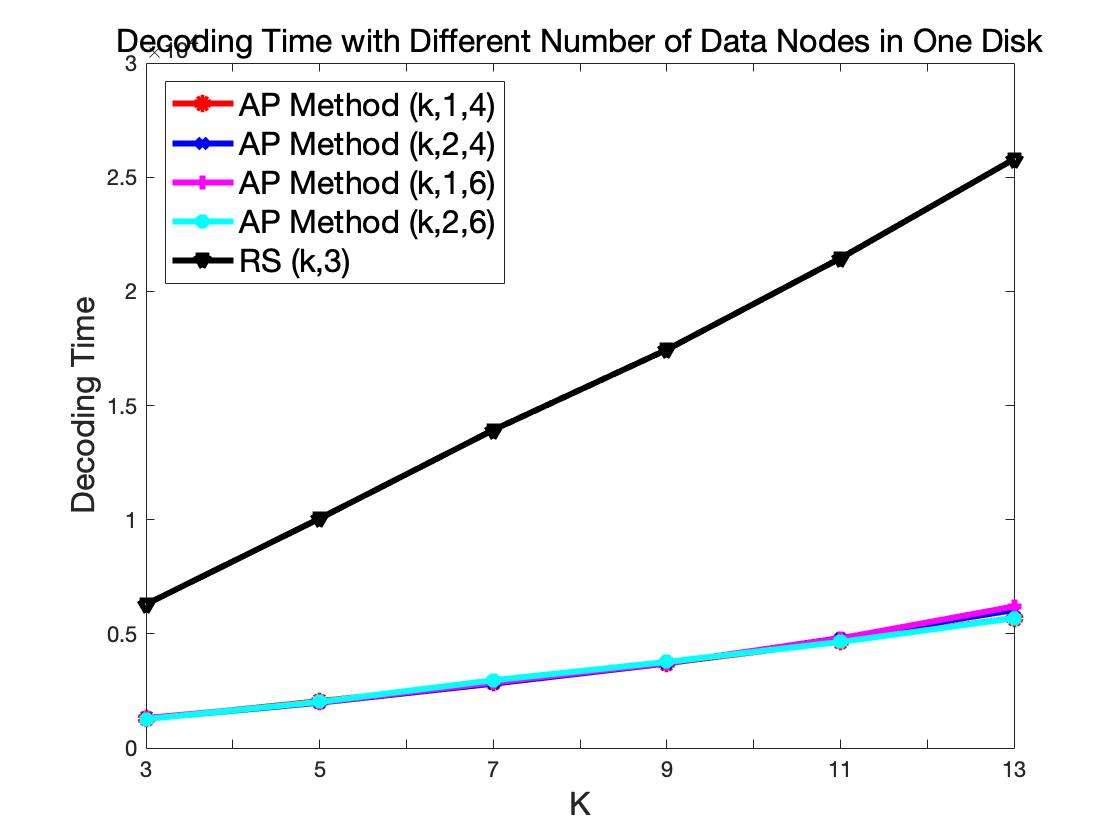
\includegraphics[width = 0.23\linewidth]{photo/experiment/Example5Modi1.jpg}
}
\subfigure[AP and STAR]{
    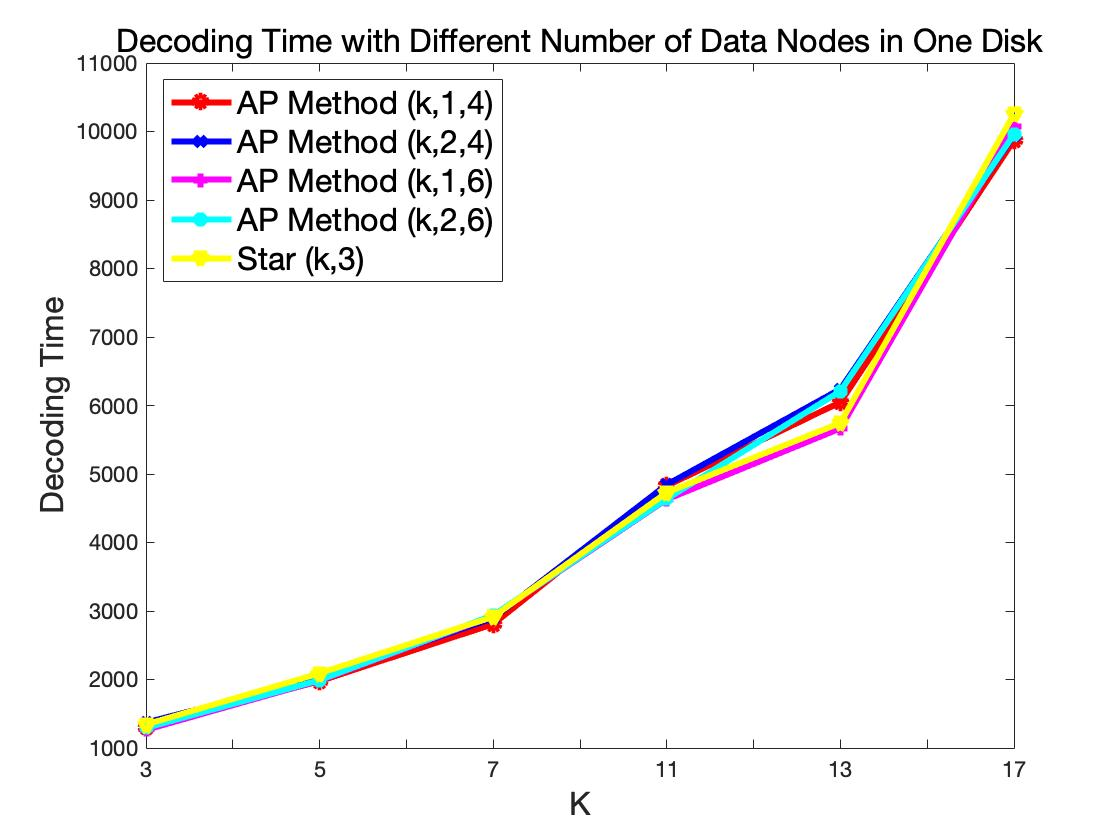
\includegraphics[width = 0.23\linewidth]{photo/experiment/Example6.jpg}
}
\subfigure[AP and TIP]{
    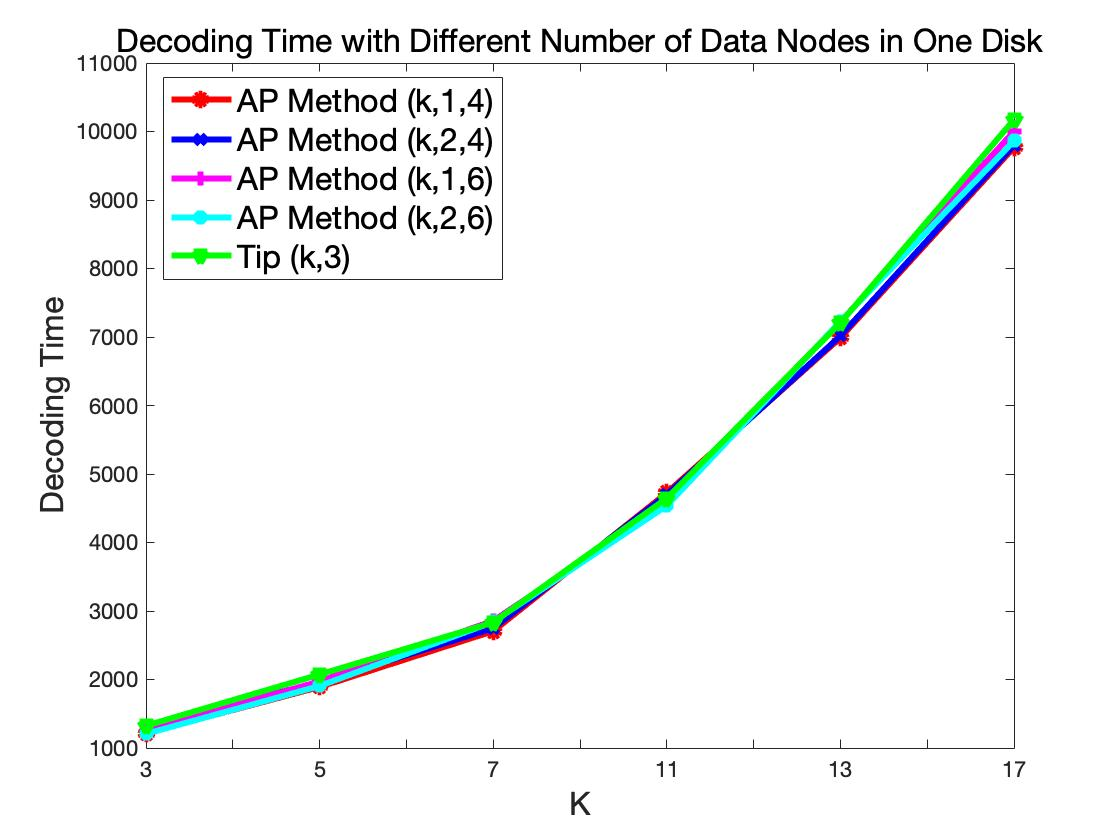
\includegraphics[width = 0.23\linewidth]{photo/experiment/Example7.jpg}
}
\subfigure[AP and LRC]{
    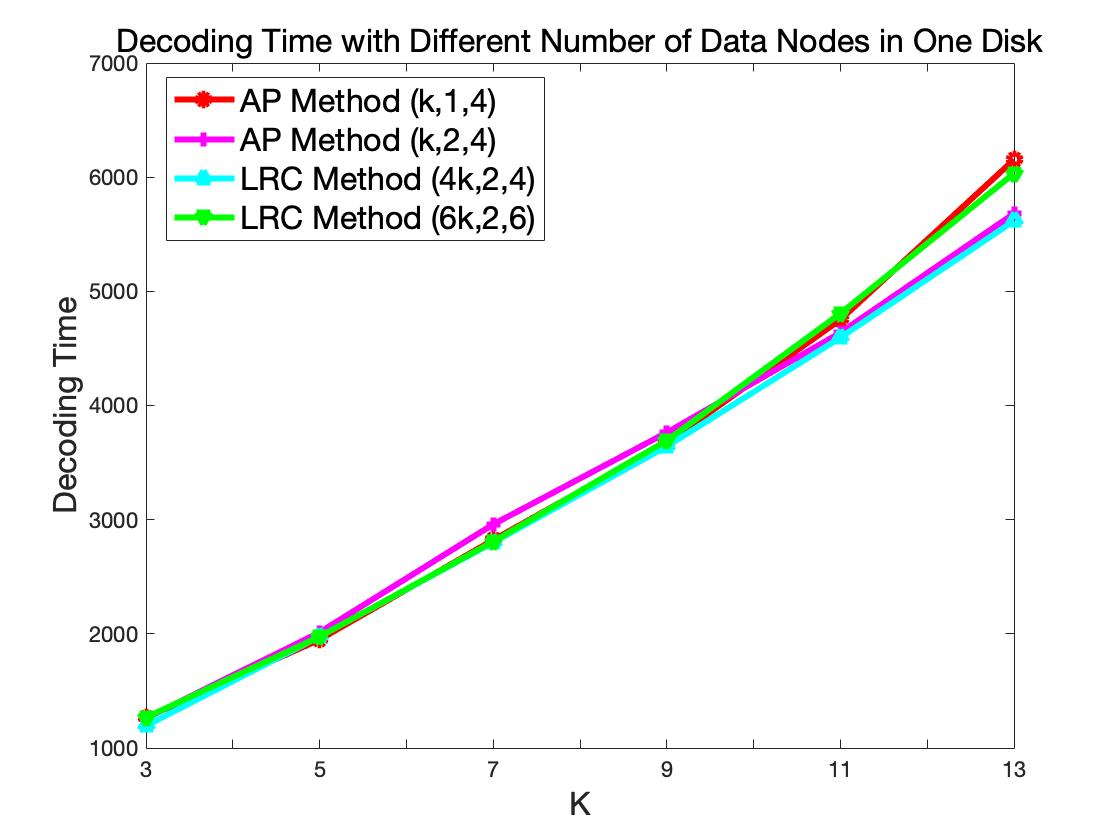
\includegraphics[width = 0.23\linewidth]{photo/experiment/Example8.jpg}
}
\caption{Decoding Time Comparison in One Disk between AP method and other method}\label{fig-decoding-1}
\end{figure*}


\begin{figure*}[]
\subfigure[AP and RS]{
    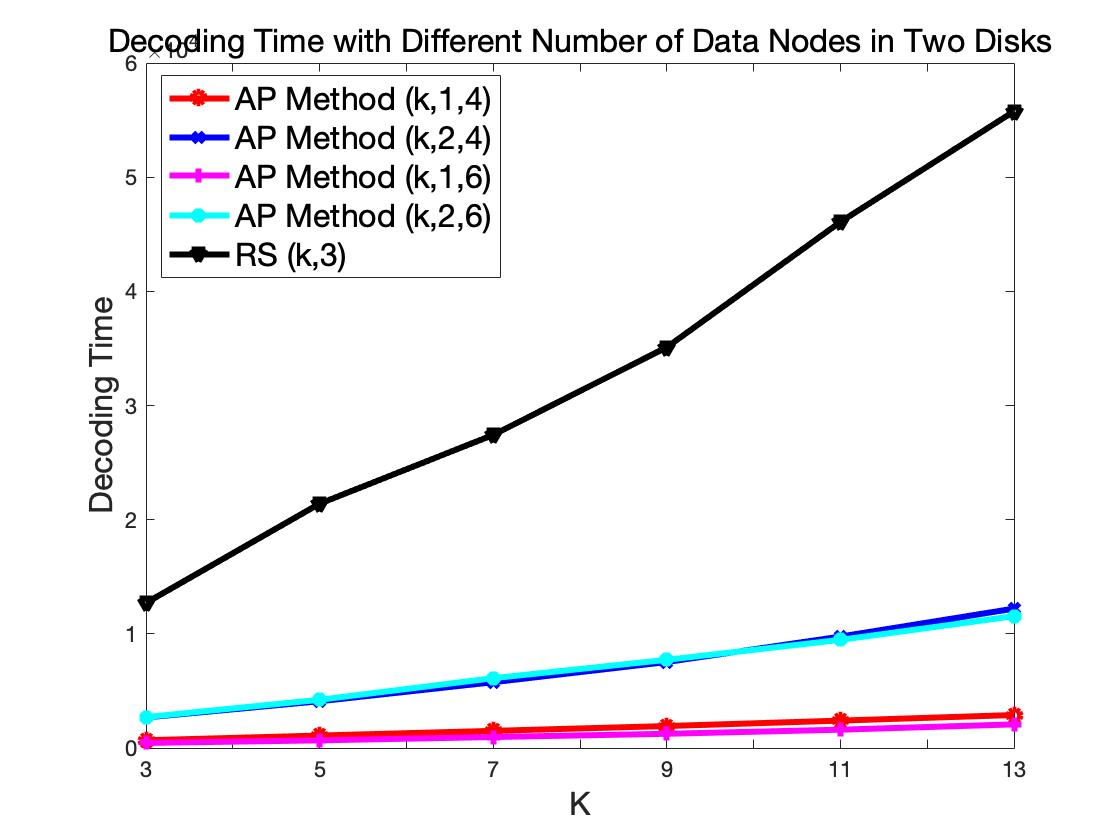
\includegraphics[width = 0.23\linewidth]{photo/experiment/Example9.jpg}
}
\subfigure[AP and STAR]{
    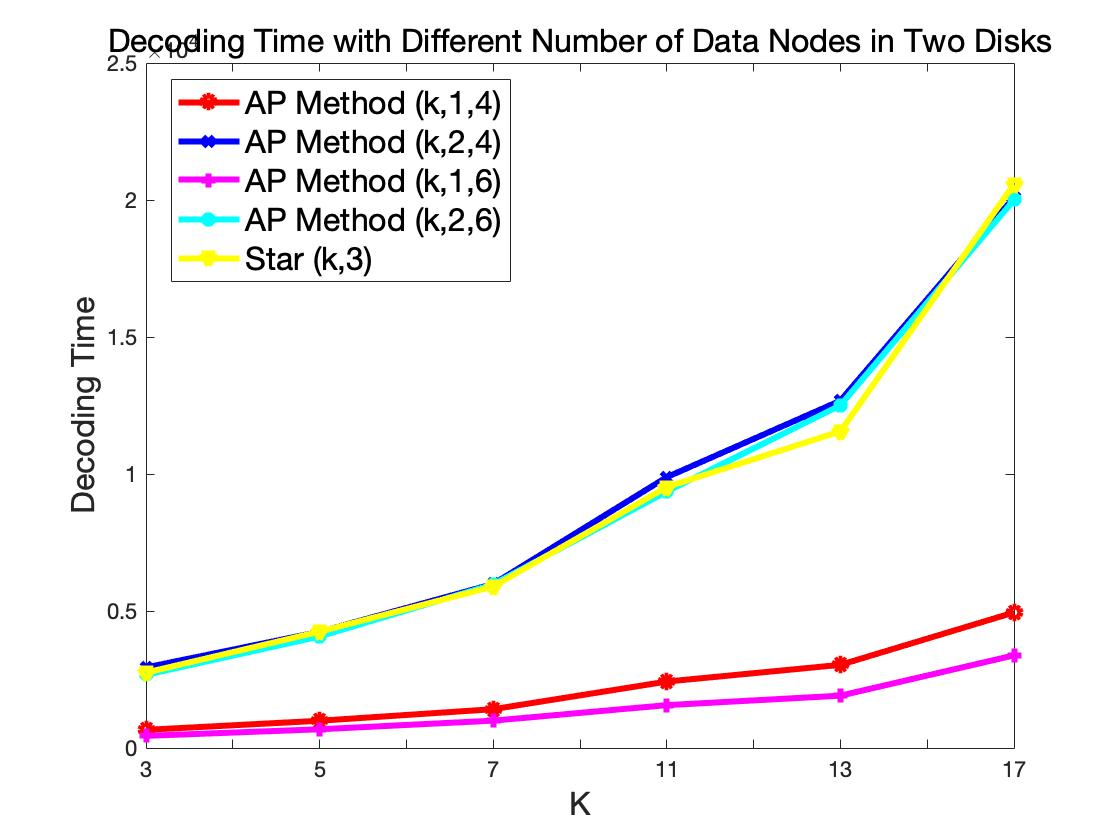
\includegraphics[width = 0.23\linewidth]{photo/experiment/Example10.jpg}
}
\subfigure[AP and TIP]{
    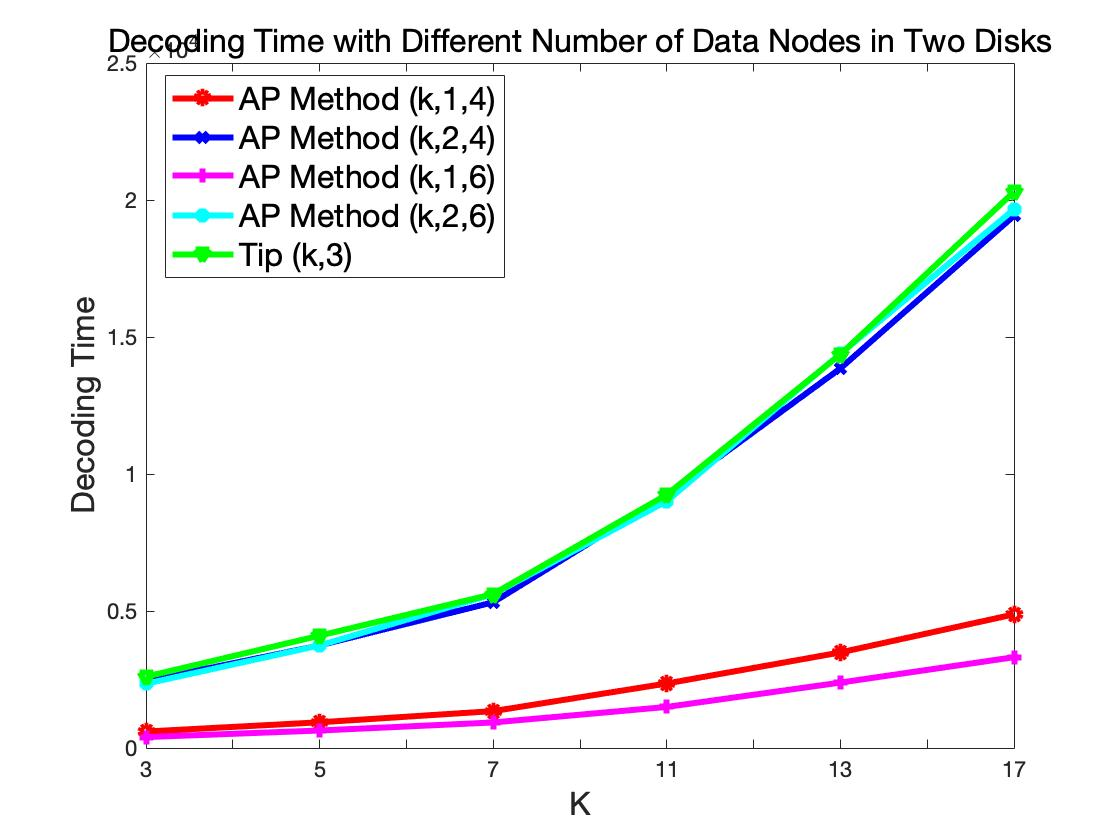
\includegraphics[width = 0.23\linewidth]{photo/experiment/Example11Modi1.jpg}
}
\subfigure[AP and LRC]{
    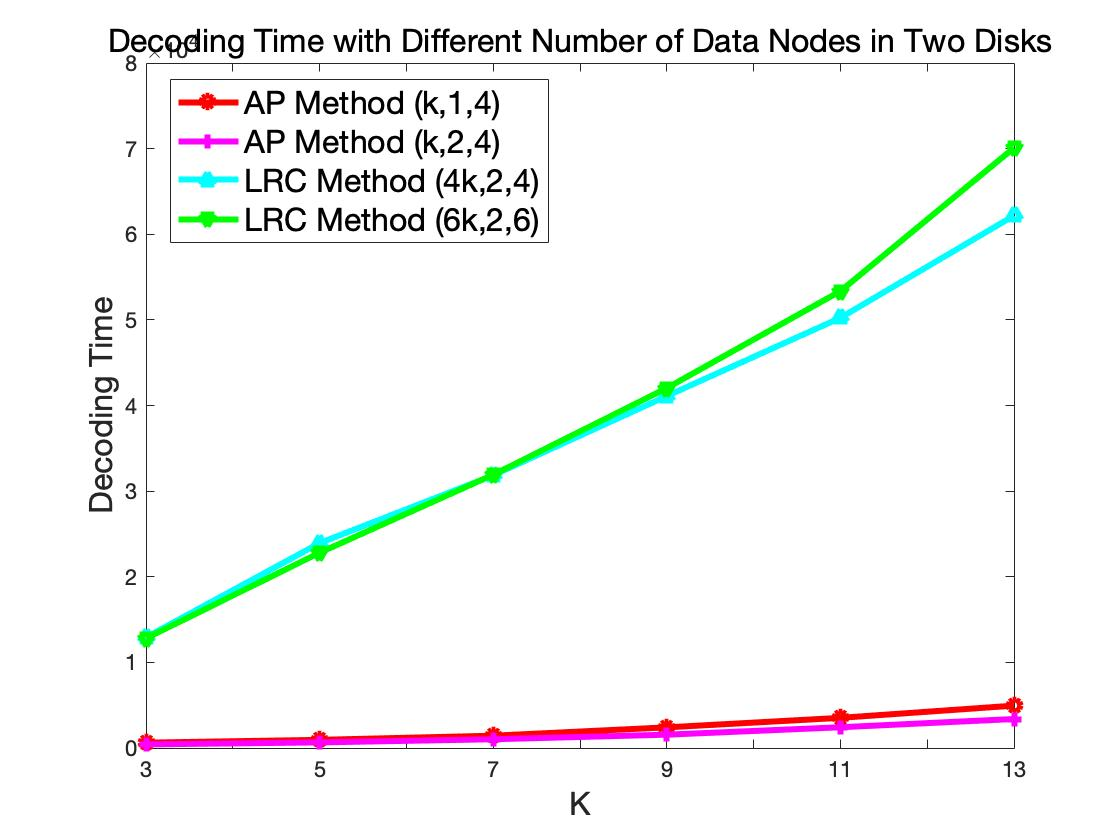
\includegraphics[width = 0.23\linewidth]{photo/experiment/Example12.jpg}
}
\caption{Decoding Time Comparison in Two Disk between AP method and other method}\label{fig-decoding-2}
\end{figure*}

According to Figure xx, we see that RS ($5$, $3$) has the longest encoding time among these methods, and the encoding time of LRC method is not short either. The methods whose encoding time is approaching to the AP method are Star and Tip. Among the AP method, AP ($5$, $1$, $6$) has the shortest encoding time.\par


\subsubsection{Decoding Time in One Disk Analysis}
From the Figure xx a), we could find out that the AP code decodes faster than RS ($k$, $3$). The rate of optimisation between AP method ($k$, $1$, $6$) and RS ($k$, $3$) is from 395.2\% (3 nodes’ case) to 353.0\% (13 nodes’ case). The Figure xx b) and c) illustrate that the effet of Star code and Tip code is similar, and there is nearly no difference among these three methods. The rate of optimisation between AP method ($k$, $2$, $6$) and Star ($k$, $3$) is from 3.867\% (3 nodes’ case) to 2.971\% (17 nodes’ case). According to Figure xx d), we could see that LRC ($4k$, $2$, $4$) decodes a bit faster than AP code, but LRC ($6k$, $2$, $6$) decodes slower than AP code. LRC ($4k$, $2$, $4$) decodes faster from 5.941\% (3 nodes’ case) to 9.542\% (13 nodes’ case) than AP ($1$, $4$); but AP ($1$, $6$) decodes faster from 0.476\% (3 nodes’ case) to 6.196\% (13 nodes’ case) than LRC ($6k$, $2$, $6$).\par


According to Figure xx, we see that RS ($5$, $3$) has the longest decoding time among these methods, while other methods decoding time in one disk have no significant difference.\par


\begin{figure*}[]
\subfigure[Encoding Time]{
    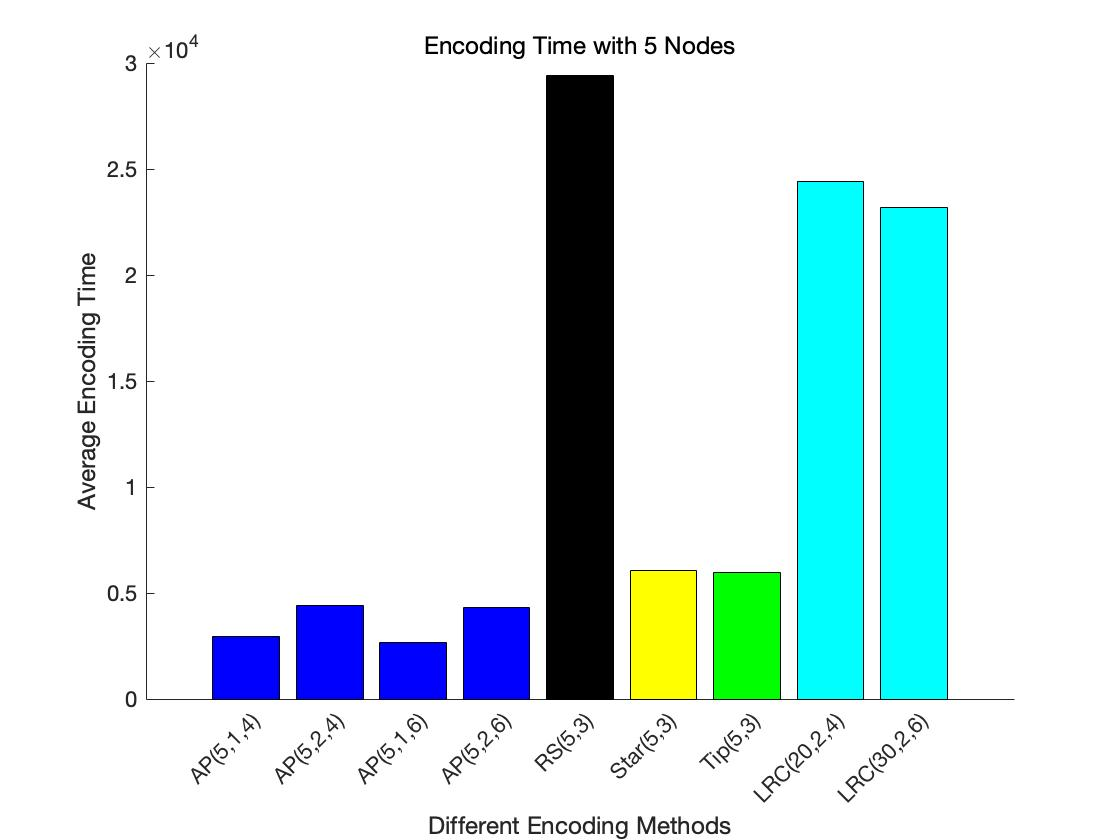
\includegraphics[width = 0.23\linewidth]{photo/experiment/BarEnT.jpg}
}
\subfigure[Decoding Time in One Node Failure]{
    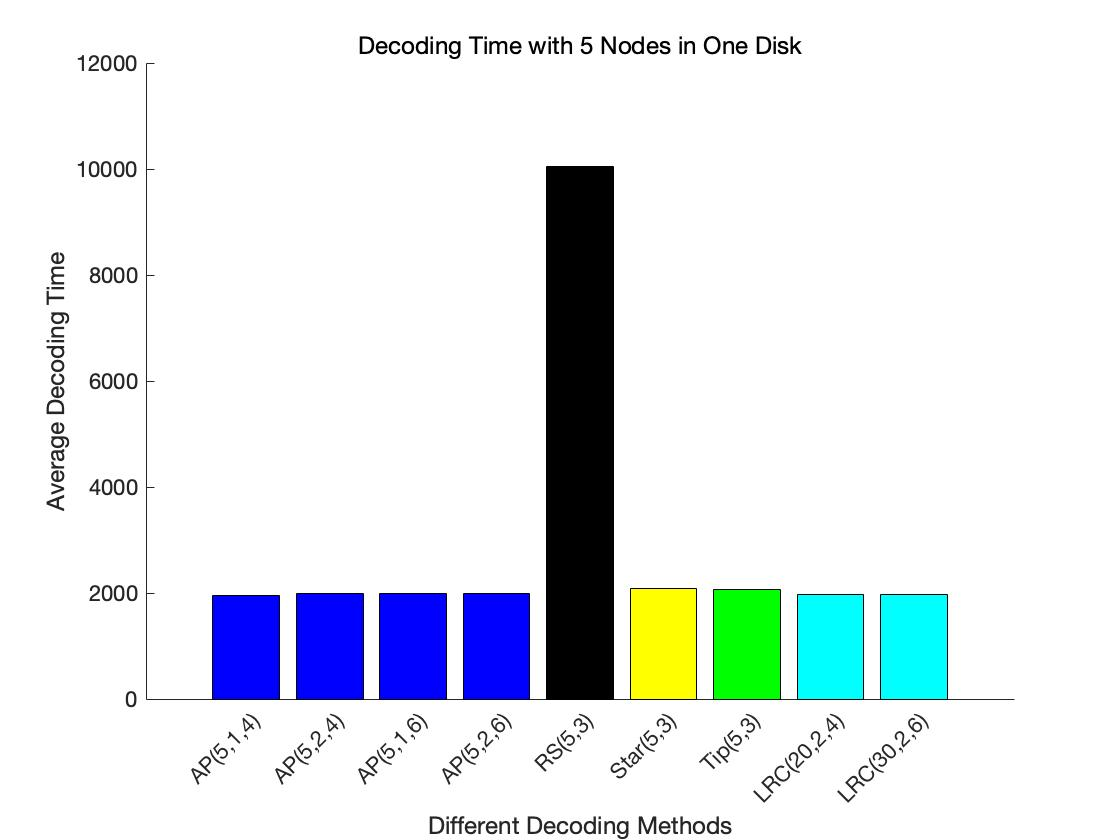
\includegraphics[width = 0.23\linewidth]{photo/experiment/BarDeT1Modi1.jpg}
}
\subfigure[Decoding Time in Two Node Failure]{
    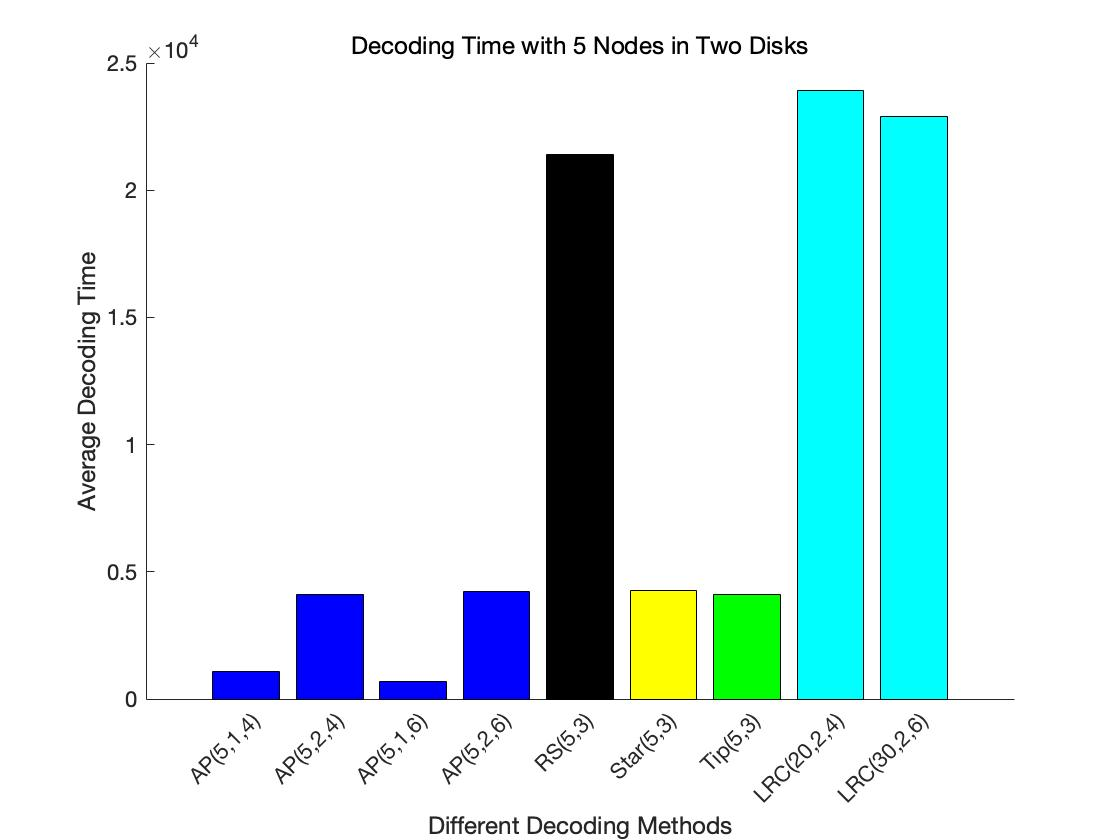
\includegraphics[width = 0.23\linewidth]{photo/experiment/BarDeT2.jpg}
}
\caption{Comparison of several matrics between different methods when number of data nodes are 5}\label{fig-BAR}
\end{figure*}


\subsubsection{Decoding Time in Two Disks Analysis}
From the Figure xx a), we could find out that the AP code decodes remarkably faster than RS ($k$, $3$) in two disks. The rate of optimisation between AP method ($k$, $1$, $6$) and RS ($k$, $3$) is from 2782.1\% (3 nodes’ case) to 2593.9\% (13 nodes’ case). The Figure xx b) and c) illustrate that the effet of Star code and Tip code for decoding in two disks is similar, and the difference between them and AP ($k$, $2$, $4$ or $6$) is not very large. However, the difference is large when it comes to AP ($k$, $1$, $6$) The rate of optimisation between AP ($k$, $1$, $6$) and Star ($k$, $3$) is from 520.8\% (3 nodes’ case) to 508.6\% (17 nodes’ case). According to Figure xx d), we could see that AP code largely reduces the decoding time in two disks in comparison to LRC method. The rate of optimisation between AP code ($k$, $1$, $4$) and LRC ($4k$, $2$, $4$) is from 1971.5\% (3 nodes’ case) to 1265.5\% (13 nodes’ case); and the rate of optimisation between AP code ($k$, $1$, $6$) and LRC ($6k$, $2$, $6$) is from 2941.3\% to 1970.7\%. Considering the optimisation rate, AP code ($k$, $1$, $6$) is the best among the four.\par

According to Figure xx, we see that RS ($5$, $3$) has the longest decoding time among these methods, the LRC method is not suitable for decoding in two disks. AP code, here, largely reduces the decoding time in two disks, while the AP ($5$, $1$, $6$) keeps the shortest decoding time.

\begin{itemize}
    \item Storage efficiency. . .
    \item Fault tolerance. . .
    \item Write overhead. . .
\end{itemize}

\subsection{Encoding Performance}
We use Approximate Code (4,2,4) and (5,1,6)...

\subsection{Recovery Time}
We use Approximate Code (4,2,4) and (5,1,6)...

\subsection{Analysis}
\section{Conclusion}\label{Conclusion}



\begin{acks}

\end{acks}



\bibliographystyle{ACM-Reference-Format}
\bibliography{ApproximateCode}

\end{document}
